\documentclass[12pt,a4paper]{report}
\usepackage[utf8]{inputenc}
\usepackage[spanish]{babel}
\usepackage{amsmath}
\usepackage{amsfonts}
\usepackage{amssymb}
\usepackage{lmodern}
\usepackage{amsmath}
\usepackage{enumerate}
\usepackage[left=2cm,right=2cm,top=2cm,bottom=2cm]{geometry}
\usepackage{graphicx}
\usepackage{mathtools}
\usepackage{stackrel}
\renewcommand{\theequation}{\arabic{equation}}
\newcounter{neq}
\providecommand{\abs}[1]{\lvert#1\rvert}
\newcommand{\QED}{\hfill \textit{\textbf{Q.E.D.}}}
\author{Agustin Curto, agucurto95@gmail.com}
\title{Resumen de teoremas para el final \\ de Matemática Discreta  II}
\date{2016}


\begin{document}
\maketitle
\tableofcontents


\chapter{Parte A}

	\section{La complejidad de EDMONS-KARP}
		\textbf{\underline{Teorema:}} La complejidad de $\langle E-K \rangle$ con $n = \abs{V}$ y $m = \abs{E}$ es $\mathcal{O}(nm^{2})$.

		\textbf{\underline{Prueba:}} Sean: $f_{0}, f_{1}, f_{2}, \; \dotsc$ \; la sucesión de flujos creados por $\langle E-K \rangle$. Es decir, el paso \textit{k} crea $f_{k}$.
			\vspace{5mm}
			\par Para cada \textit{k} definimos funciones:
			\begin{itemize}
				\item $d_{k}(x) =$ \textquotedblleft distancia\textquotedblright \; entre \textit{s} y x en el paso \textit{k}, en caso de existir, si no $\infty$.
				\item $b_{k}(x) =$ \textquotedblleft distancia\textquotedblright \; entre x y \textit{t} en el paso \textit{k}, en caso de existir, si no $\infty$.
			\end{itemize}

			\textquotedblleft Distancia\textquotedblright: longitud del menor camino aumentante.

			\vspace{5mm}
			\par Sabemos que las distancias de $\langle E-K \rangle$ no disminuyen en pasos sucesivos, como esto será útil para esta demostración llamaremos $\circledast$ a la demostración de:
				\[ d_{k}(x) \leq d_{k+1}(x) \]
				\[ b_{k}(x) \leq b_{k+1}(x) \]

			\par Llamemos \textit{\underline{crítico}} a un lado disponible en el paso \textit{k} pero no disponible en el paso \textit{k + 1}. Es decir, si \textit{xy} es un lado $\Rightarrow$ \textit{xy} se satura ó \textit{yx} se vacía en el paso \textit{k}.
			\begin{enumerate}
				\item Supongamos que al construir $f_{k}$ el lado \textit{xy} se vuelve crítico, el camino: \textit{s} $\dotsc$ x, y $\dotsc$ \textit{t} se usa para construir $f_{k}$.
				\begin{eqnarray}
					\nonumber d_{k}(\textit{t}) &=& d_{k}(x) + b_{k}(x) \\
					\nonumber &=& d_{k}(x) + b_{k}(y) + 1
				\end{eqnarray}

				\item Para que \textit{xy} pueda ser \textit{crítico} nuevamente debe ser usado en la otra dirección. Sea \textit{l} el paso posterior a \textit{k} en el cual se usa el lado en la otra dirección, el camino \textit{s} $\dotsb$ y, x $\dotsb$ \textit{t} se usa para construir $f_{l}$.
				\begin{eqnarray}
					\nonumber d_{l}(t) &=& d_{l}(x) + b_{l}(x) \\
					\nonumber &=& d_{l}(y) + 1 + b_{l}(x)
				\end{eqnarray}
			\end{enumerate}

			\par Entonces:
			\begin{equation*}
				\textup{De (1) y (2) } \Rightarrow
	  		\left \lbrace
	  		\begin{array}{l}
					d_{k}(y) = d_{k}(x) + 1 \; \; \star \\
	    		d_{l}(x) = d_{l}(y) + 1 \; \; \; \dag
	  		\end{array}
	  		\right.
			\end{equation*}

			\par Luego:
			\begin{eqnarray}
				\nonumber d_{l}(t) &=& d_{l}(x) + b_{l}(x) \\
				\nonumber &=& d_{l}(y) + 1 + b_{l}(x) \qquad\qquad\qquad\;\text{Por } \dag \\
				\nonumber & \geq & d_{k}(y) + 1 + b_{k}(x) \qquad\qquad\qquad\text{Por} \circledast \\
				\nonumber &=& d_{k}(x) + 1 + 1 + b_{k}(x) \;\qquad\qquad\text{Por} \star \\
				\nonumber &=& d_{k}(\textit{t}) + 2 \\
				\nonumber \therefore d_{l}(\textit{t}) & \geq & d_{k}(\textit{t}) + 2
			\end{eqnarray}

			\vspace{5mm}
			\par Por lo tanto cuando un lado se vuelve crítico recien puede volver a usarse cuando la distancia de \textit{s} a \textit{t} haya aumentado en por lo menos 2. Puede existir $\mathcal{O}(n/t)$ tales aumentos, es decir:
				\[ \# \textup{ Veces que un lado puede volverse crítico } = \mathcal{O}(n). \]

			\begin{eqnarray}
				\nonumber \; \therefore Complejidad(\langle E-K\rangle) &=& (\# pasos) * Complejidad(1 \; \textit{paso}) \\
				\nonumber &=& (\# \textup{veces que un lado se vuelve crítico}) * (\# lados) * Complejidad(BFS) \\
				\nonumber  &=& \mathcal{O}(n) * \mathcal{O}(m)* \mathcal{O}(m) \\
				\nonumber &=& \mathcal{O}(nm^{2})
			\end{eqnarray}

		\QED

	\pagebreak
	\section{Las distancias de EDMONS-KARP no disminuyen en pasos sucesivos}
		\textbf{\underline{Teorema:}} Sean: $f_{0}, f_{1}, f_{2}, \; \dotsc$ \; la sucesión de flujos creados por $\langle E-K\rangle$. Es decir, el paso \textit{k} crea $f_{k}$.

			\vspace{5mm}
			\par Para cada \textit{k} definimos funciones:

			\begin{itemize}
				\item $d_{k}(x) =$ \textquotedblleft distancia\textquotedblright \; entre \textit{s} y x en el paso \textit{k} en caso de existir, si no $\infty$.
				\item $b_{k}(x) =$ \textquotedblleft distancia\textquotedblright \; entre x y \textit{t} en el paso \textit{k} en caso de existir, si no $\infty$.
			\end{itemize}

			\textquotedblleft Distancia\textquotedblright: longitud del menor camino aumentante.

			\vspace{5mm}
			\par Queremos probar que:
			\begin{enumerate}
				\item $d_{k}(x) \leq d_{k + 1}(x)$
				\item $b_{k}(x) \leq b_{k + 1}(x)$
			\end{enumerate}

		\textbf{\underline{Prueba:}} Lo probaremos por inducción y solo para $d_{k}$ ya que para $b_{k}$ la prueba es análoga.
			\[ \textup{HI: H(i) } = \lbrace\forall_{z}: d_{k + 1}(z) \leq \textit{i}, \textup{ vale } d_{k}(z) \leq d_{k + 1}(z)\rbrace \]

			\begin{enumerate}
				\item \underline{Caso Base:} \begin{tabular}{|c|} \hline i = 0 \\\hline \end{tabular} \qquad $H(0) = \lbrace\forall_{z}: d_{k + 1}(z) \leq 0, \textup{ vale } d_{k}(z) \leq d_{k + 1}(z)  \rbrace$
					\par Pero $d_{k + 1}(z) \leq 0 \Rightarrow z = \textit{s}$, entonces:
					\begin{eqnarray}
						\nonumber d_{k}(z) &=& d_{k}(s) \\
						\nonumber &=& 0 \\
						\nonumber &\leq & d_{k + 1}(s) \\
						\nonumber &=& d_{k + 1}(z) \\
						\nonumber \therefore d_{k}(z) & \leq & d_{k + 1}(z)
					\end{eqnarray}
				\item \underline{Caso Inductivo:} Supongamos ahora que vale H(\textit{i}), veamos que vale H(\textit{i + 1}).
					\par Sea \textit{z} con $d_{k + 1}(z) \leq \textit{i+1}$, si $d_{k + 1}(z) \leq \textit{i}$ vale H(\textit{i}) para \textit{z}.
					\par \begin{center} $\therefore \; d_{k}(z) \leq d_{k + 1}(z) $ \end{center}
					\par Supongamos que \begin{tabular}{|c|} \hline $d_{k + 1}(z) = i + 1$ \\\hline \end{tabular} $\circledast$
					\par Entonces existe un camino aumentante, relativo a $f_{k}$, de la forma: $s = z_{0},  \; \dotsc \; z_{i}, \; z_{i + 1} = z$.
					\par Sea \begin{tabular}{|c|} \hline $x = z_{i}$ \\ \hline \end{tabular}

					\begin{itemize}
						\item \underline{Caso 1:} Existe algun camino aumentante, relativo a $f_{k - 1}$, de la forma $s, \; \dotsc \; x, \; z$.
							\begin{center}
								$\therefore d_{k}(z) \leq d_{k}(x) + 1$
							\end{center}

							\vspace{2mm}
							\par Pues al haber un camino $\underbrace{s, \; \dotsc \; x,}_{d_{k}(x)} \; z$, llamemosle A, de longitud $d_{k}(x) + 1$ entre \textit{s} y \textit{z}, sabemos que el mínimo de todos los caminos de \textit{s} a \textit{z} serán $\leq$ A.
						\item \underline{Caso 2:} No existe un camino aumentante, relativo a $f_{k - 1}$, pero si existe un camino aumentante relativo a $f_{k}$. Por lo tanto el lado \textit{xz} no esta \textquotedblleft disponible\textquotedblright \; en el paso \textit{k}, ya que \textit{xz} está saturado, o bien \textit{zx} está vacío relativo a $f_{k - 1}$. Es decir:
							\vspace{5mm}
							\begin{enumerate}[1)]
								\item $f_{k - 1}(\overrightarrow{xz}) = Cap(\overrightarrow{xz})$ pero $f_{k}(\overrightarrow{xz}) < Cap(\overrightarrow{xz}), \; f_{k}$ devuelve flujo por $\overrightarrow{xz}$ ó
								\item $f_{k - 1}(\overrightarrow{zx}) = 0$ pero $f_{k}(\overrightarrow{zx}) > 0, \; f_{k}$ manda flujo por $\overrightarrow{zx}$.
							\end{enumerate}

							\vspace{5mm}
							\par Para construir $f_{k}$ usamos un camino de la forma $s, \; \dotsc \; z, \; x$.
							\par Como $\langle E-K \rangle$ funciona con BFS, ese camino usado para construir $f_{k}$ debe ser de longitud mínima. Es decir:
							\begin{eqnarray}
								\nonumber d_{k}(x) &=& d_{k}(z) + 1 \\
								\nonumber \Rightarrow d_{k}(z) &=& d_{k}(x) - 1 \\
								\nonumber &\leq & d_{k}(x) + 1
							\end{eqnarray}
					\end{itemize}

				\underline{Conclusión:} En cualquiera de los dos casos tenemos:
				\begin{center}
					\begin{tabular}{|c|} \hline $d_{k}(z) \leq d_{k}(x) + 1$ \\\hline \end{tabular} (1)
				\end{center}

				\par Ahora bien:
				\begin{eqnarray}
					\nonumber d_{k + 1}(x) &=& d_{k + 1}(z_{i}) \\
					\nonumber &=& i \qquad \qquad \; \; \; (2) \\
					\nonumber &\Rightarrow & \textup{H(\textit{i}) vale para x.} \\
					\nonumber \therefore \; d_{k}(x) & \leq & d_{k + 1}(x) \qquad (3)
				\end{eqnarray}

				\par Por lo tanto:
				\begin{eqnarray}
					\nonumber d_{k}(z) &\leq & d_{k}(x) + 1 \qquad \qquad \textup{ Por } (1) \\
					\nonumber &\leq & d_{k + 1}(x) + 1 \qquad \; \; \; \; \textup{ Por (3)} \\
					\nonumber &=& i + 1 \qquad \qquad \qquad \textup{ Por } (2) \\
					\nonumber &=& d_{k + 1}(z) \qquad \qquad \; \; \; \textup{ Por} \circledast \\
					\nonumber & \Rightarrow & \textup{H(i + 1) vale.}
				\end{eqnarray}
			\end{enumerate}

		\QED

	\pagebreak
	\section{La complejidad de DINIC}
		\textbf{\underline{Teorema:}} La complejidad del algoritmo de Dinic es $\mathcal{O}(n^{2}m)$.

		\textbf{\underline{Prueba:}} Como Dinic es un algoritmo que trabaja con networks auxiliares y vimos que la distancia entre \textit{s} y \textit{t} en networks auxiliares consecutivos aumenta y puede ir a lo sumo entre 1 y $n - 1$ entonces hay a lo sumo $\mathcal{O}(n)$ networks auxiliares.
			\[ \textup{Complejidad(Dinic) } = \mathcal{O}(n) * \textup{ Complejidad(Paso Bloqueante de Dinic)} \]
			\par Para probar que la complejidad de Dinic es $\mathcal{O}(n^{2}m)$ debemos probar que la complejidad del paso bloqueante es $\mathcal{O}(nm)$.
			\par Sean:
			\begin{itemize}
				\item A $=$ Avanzar()
				\item R $=$ Retroceder()
				\item I $=$ IncrementarFlujo() + Inicialización()
			\end{itemize}

			\par Una corrida de Dinic luce como:
			\begin{center}
				AA$\; \dotsc \;$AIAAARA$\; \dotsc \;$AIAARAAARR$\; \dotsc \;$IA$\; \dotsc \;$
			\end{center}

			\par Dividamos la corrida en subpalabras del tipo:
			\begin{equation*}
		  	\left.
		  	\begin{array}{l}
		    	\underbrace{AA \; \dotsc \; A}_{Todas \; A's}R \\
		    	\underbrace{AA \; \dotsc \; A}_{Todas \; A's}I
		  	\end{array}
		  	\right\rbrace
		  	\textup{ Sea X = I o R}
			\end{equation*}
			\par \textbf{Nota:} el número de A's puede ser 0.
			\vspace{1.5mm}
			\par Debemos determinar:
			\begin{enumerate}
				\item \textbf{Cantidad de subpalabras}
					\begin{equation*}
						\left.
						\begin{array}{l}
							X = R: \textup{ borramos un lado} \\
							X = I \; : \textup{ borramos al menos un lado}
						\end{array}
						\right\rbrace
						\Rightarrow \textup{ Cada X borra al menos un lado}
					\end{equation*}
					\begin{center}
						$\therefore$ hay $\leq m$ palabras de la forma $A \dotsc A X$
					\end{center}
				\item \textbf{Complejidad de cada subpalabra}
					\par Recordemos que:
					\begin{equation*}
						\textup{A:}
						\left[
						\begin{array}{l}
							P[i + 1] = \textup{algún elemento de } \Gamma^{+}(P[i]) \\
							i = i + 1
						\end{array}
						\right.
					\end{equation*}
					\[ \Rightarrow \textup{ A es } \mathcal{O}(1) \]

					\begin{equation*}
						\textup{R:}
						\left[
						\begin{array}{l}
							\textup{Borrar } P[i - 1]P[i] \textup{ del NA} \\
							i = i - 1
						\end{array}
						\right.
					\end{equation*}
					\[ \Rightarrow \textup{ R es } \mathcal{O}(1) \]

					\begin{equation*}
						\textup{I:}
						\left[
						\begin{array}{l}
							\textup{Recorre un camino de longitud } \leq n
						\end{array}
						\right.
					\end{equation*}
					\[ \Rightarrow \textup{ I es } \mathcal{O}(n) \]

					\par Luego:
					\begin{eqnarray}
						\nonumber Complejidad(X) &=& \mathcal{O}(n) \\
						\nonumber \therefore Complejidad (\underbrace{A \; \dotsc \; A}_{j \; veces}X) &=&\mathcal{O}(j) + \mathcal{O}(n)
					\end{eqnarray}

					\par Como cada Avanzar() mueve el pivote un nivel más cerca de \textit{t} entonces hay a lo sumo \textit{n} Avanzar() antes de un R o un I $\Rightarrow j\leq$ n.
					\[ \therefore \; Complejidad(A \dotsc AX) = \mathcal{O}(n) + \mathcal{O}(n) = \mathcal{O}(n)\]
			\end{enumerate}

			\par De (1) y (2):
			\begin{eqnarray}
				\nonumber \textup{Complejidad(Paso Bloqueante de Dinic)} &=& \# (A \dotsc A X) * \textup{Complejidad} (A \dotsc A X) \\
				\nonumber &=& m * \mathcal{O}(n) \\
				\nonumber &=& \mathcal{O}(m*n)
			\end{eqnarray}

		\QED


	\section{La complejidad de WAVE}
		\textbf{\underline{Teorema:}} La complejidad del algoritmo de Wave es $\mathcal{O}(n^{3})$.

		\textbf{\underline{Prueba:}} Como Wave es un algoritmo que trabaja con networks auxiliares y vimos que la distancia entre \textit{s} y \textit{t} en networks auxiliares consecutivos aumenta y puede ir a lo sumo entre 1 y $n - 1$ entonces hay a lo sumo $\mathcal{O}(n)$ networks auxiliares.
			\begin{center}
				Complejidad(Wave)$ = \mathcal{O}(n) \; *$ Complejidad(Paso Bloqueante de Wave)
			\end{center}

			\par Para probar que la complejidad de Wave es $\mathcal{O}(n^{3})$ debemos probar que complejidad del paso bloqueante es $\mathcal{O}(n^{2})$. El paso bloqueante de Wave consiste en una serie de:
			\begin{itemize}
				\item Olas hacia adelante: Sucesión de \textbf{fordwardbalance} (FB)
				\item Olas hacia atrás: Sucesión de \textbf{backwardbalance} (BB)
			\end{itemize}

			\par Cada FB y BB es una sucesión de \textquotedblleft \textbf{buscar vecinos}\textquotedblright \; y \textquotedblleft \textbf{procesar}\textquotedblright \; el lado resultante. Estos "procesamientos" \; son complicados pero $ \mathcal{O}(1)$.
			\[ \therefore \textup{ Complejidad(Paso Bloqueante de Wave) } = \# \textup{ \textquotedblleft procesamientos de lado\textquotedblright} \]

			\par Los \textquotedblleft procesamientos\textquotedblright \; de lados los podemos dividir en dos categorías:
			\begin{enumerate}
				\item Aquellos procesamientos que saturan o vacian el lado. Denotaremos \textquotedblleft T\textquotedblright \; al número de estos procesamientos.
				\item Aquellos procesamientos que no saturan ni vacian el lado. Denotaremos \textquotedblleft Q\textquotedblright \; al número de estos procesamientos.
			\end{enumerate}
			\par Por lo tanto queremos acotar $T + Q$.

			\pagebreak
			\textbf{Complejidad de T:}
			\begin{itemize}
				\item ¿Puede un lado $\overrightarrow{xy}$ saturado volver a saturarse?
					\par Para poder volver a \underline{saturarse} primero tiene que vaciarse aunque sea un poco, es decir, antes de poder volver a saturarlo \textit{y} debe devolver flujo a \textit{x}, pero para que en Wave \textit{y} le devuelva flujo a \textit{x} debe ocurrir que \textit{y} esté bloqueado (porque BB(y) solo se ejecuta si \textit{y} está bloqueado), pero si \textit{y} está bloqueado \textit{x} no puede mandarle flujo nunca más.
					\[ \therefore \overrightarrow{xy} \textup{ no puede resaturarse } \]
					\par \underline{Conclusión 1:} Los lados se saturan solo una vez.
				\item ¿Puede un lado $\overrightarrow{xy}$ vaciado completamente volver a vaciarse?
					\par Para poder volver a \underline{vaciarse} como está vacío completamente, primero hay que mandar flujo, pero si lo vacié, \textit{y} está bloqueado por lo que \textit{x} no puede mandar flujo.
					\[ \therefore \overrightarrow{xy} \textup{ no puede volver a vaciarse } \]
					\par \underline{Conclusión 2:} Los lados se vacían completamente a lo sumo una vez.

				\par Las conclusiones (1) y (2) implican que \begin{tabular}{|c|} \hline $T \leq 2 \; m$ \\\hline \end{tabular}
			\end{itemize}

			\textbf{Complejidad de Q:}
				\vspace{3mm}
				\par En cada FB a lo sumo un lado no se satura y en cada BB a lo sumo un lado no se vacía completamente.
				\[ \therefore Q \leq \# \textup{ Total de FB's y BB's} \]
				\begin{itemize}
					\item \# FB's en cada ola hacia adelante es $\leq$ \textit{n} (un FB por vértice)
					\item \# BB's en cada ola hacia atrás es $\leq$ \textit{n} (un BB por vértice)

					\vspace{5mm}
					\par $\therefore$ Total de FB's y BB's $\leq 2 n \; \#$Total de ciclos de \textquotedblleft ola adelante $-$ ola hacia atrás\textquotedblright
	 			\end{itemize}

				\par Ahora bien, en cada ola hacia adelante, pueden o no, bloquearse algunos vértices. Si no se bloquea ningún vértice, entonces todos los vértices ($\neq$ \textit{s, t}) quedan balaceados por lo que estamos en la última ola. Luego en toda ola que no sea la última se bloquea al menos un vértice ($\neq$ \textit{s, t}).
				\begin{center}
					$\therefore \; \#$ Total de ciclos es $\leq (n - 2) + 1 = n - 1$ \\
					\vspace{3mm}
					$\Rightarrow$ \begin{tabular}{|c|} \hline $Q \; \leq 2 n \; (n - 1) = \mathcal{O}(n^{2})$ \\ \hline \end{tabular}
				\end{center}

				\begin{eqnarray}
					\nonumber \therefore \; T + Q &\leq & 2 m + \mathcal{O}(n^{2}) \\
					\nonumber &=& \mathcal{O}(m) + \mathcal{O}(n^{2}) \\
					\nonumber &=& \mathcal{O}(n^{2})
				\end{eqnarray}

		\QED

	\section{La distancia entre NA sucesivos aumenta}
		\textbf{\underline{Teorema:}} Sea A un NA (network auxiliar) y sea $A^{*}$ el siguiente NA. Sean $d(x)$ y $d^{*}(x)$ las distancias de \textit{s} a x en A y $A^{*}$ respectivamente, entonces: $d(t) < d^{*}(t)$.

		\textbf{\underline{Prueba:}} Por la prueba de $\langle E-K \rangle$ sabemos que $d(t) \leq d^{*}(t)$ pero queremos ver el $<$.
			\par Sea:
			\[ s = x_{0}, x_{1}, \dotsc x_{r} = t \]
			\par un camino dirigido en $A^{*}$.
			\par Ese camino \begin{tabular}{|c|} \hline NO EXISTE \\\hline \end{tabular} en A ya que para pasar de A a $A^{*}$ debemos bloquear todos los caminos dirigidos de A. Por lo tanto si ese camino estuviese en A, Dinic lo habría bloqueado y no estaría en $A^{*}$.

			\vspace{5mm}
			\textbf{¿Cuáles son las razones posibles para que no esté en A?}
				\begin{enumerate}
					\item Puede faltar un vértice, es decir $\exists i : x_{i} \; \nexists \; V(A)$ entonces:
						\begin{eqnarray}
							\nonumber d(t) &\leq & d(x_{i}) \; \; \; \textup{ Por def de } d_{k}(x), \; \nexists \; \infty \\
							\nonumber &\leq & d^{*}(x_{i}) \; \; \textup { Por } \langle E-K \rangle \\
							\nonumber &< & d^{*}(t) \; \; \; \; \textup{ Porque } x_{i} \textup{ esta antes que t}
						\end{eqnarray}
						$\qquad\qquad\qquad\qquad\;$
						\begin{tabular}{|c|} \hline $\therefore \; d(t) < d^{*}(t)$ \\\hline \end{tabular}
					\item Están todos los vértices pero falta una arista, es decir $\exists i : \overrightarrow{x_{i}x_{i + 1}} \; \notin E(A)$.
						\begin{enumerate}[a)]
							\item $\overrightarrow{x_{i}x_{i + 1}}$ no está porque corresponde a un lado vacío o saturado en NA, es decir $\overrightarrow{x_{i}x_{i + 1}}$ no está en el residual que dá origen a A pero si está en el residual que dá origen a $A^{*}$.
								\par Para que esto pase se tiene que haber usado el lado $\overrightarrow{x_{i + 1}x_{i}}$ en A. Luego podemos concluir, por la prueba de $\langle E-K\rangle$ que:
								\[ d^{*}(t) \geq d(t) + 2 > d(t) \]
								$\qquad\qquad\qquad\qquad\qquad\qquad$
								\begin{tabular}{|c|} \hline $\therefore \; d(t) < d^{*}(t)$ \\\hline \end{tabular}
							\item $\overrightarrow{x_{i}x_{i + 1}}$ si está en el residual pero:
								\begin{tabular}{|c|} \hline $d(x_{i+1}) \neq d(x_{i}) +1 $ \\ \hline \end{tabular} (1)

								\vspace{5mm}
								\par Pero como $\overrightarrow{x_{i}x_{i + 1}}$ está en el residual entonces:
								\begin{tabular}{|c|} \hline $d(x_{i+1}) \leq d(x_{i}) +1 $ \\ \hline \end{tabular} (2)

								\vspace{5mm}
								\par De (1) y (2) tenemos que: \begin{tabular}{|c|} \hline $d(x_{i+1}) < d(x_{i}) +1 $ \\ \hline \end{tabular} $\circledast$

								\vspace{3mm}
								\par Entonces:
								\begin{eqnarray}
									\nonumber d(t) &=& d(x_{i + 1}) + b(x_{i + 1}) \qquad\;\;\;\;\; \textup{Por } \langle E-K\rangle \\
									\nonumber &\leq & d(x_{i + 1}) + b^{*}(x_{i + 1}) \qquad\;\;\;\; \textup{Por } \langle E-K\rangle \\
									\nonumber &<& d(x_{i}) + 1 + b^{*}(x_{i + 1}) \qquad\; \textup{Por } \circledast \\
									\nonumber &\leq & d^{*}(x_{i}) + 1 + b^{*}(x_{i + 1}) \qquad \textup{Por } \langle E-K\rangle \\
									\nonumber &=& d^{*}(x_{i + 1}) + b^{*}(x_{i + 1}) \qquad\;\;\; \textup{Por } (\dag) \\
									\nonumber &=& d^{*}(t)
								\end{eqnarray}
								$\qquad\qquad\qquad\;\;\;$
								\begin{tabular}{|c|} \hline $\therefore \; d(t) < d^{*}(t)$ \\ \hline \end{tabular}

								\vspace{5mm}
								\par ($\dag$): Ya que $s, \; x_{1}, \; \dotsc \; x_{r}$ es un camino en A*.
						\end{enumerate}
			\end{enumerate}

		\QED


\chapter{Parte B}

	\section{2-COLOR es polinomial}
		\textbf{\underline{Teorema:}} 2-Color es polinomial, es decir, existe un algoritmo polinomial que lo resuelve.

		\textbf{\underline{Prueba:}} Consideremos el siguiente algoritmo con entrada $G = (V, E)$ con $n = \abs{V}$ y $m = \abs{E}$.

			\vspace{5mm}
			\par \textbf{Algoritmo:}
			\par Por cada COMPONENTE CONEXA de G:
				\begin{enumerate}
					\item Elegir x
					\item Correr BFS(x)
					\item Colorear vertices con: $\qquad	C(v) = Nivel_{BFS(x)}(v) \; mod \; 2$
					\item Chequear que el coloreo de (3) sea propio. Si lo es, RETURN \textquotedblleft SI\textquotedblright, si no lo es, RETURN \textquotedblleft NO\textquotedblright.
				\end{enumerate}

			\par Veamos ahora que el algoritmo es correcto y que su complejidad es polinomial.
			\begin{itemize}
				\item \underline{Complejidad Polinomial:}
					\begin{itemize}
						\item (1) es $\mathcal{O}(1)$.
						\item (2) + (3) es $\mathcal{O}(m + a)$ recorrer todas las aristas, donde $a = \#$vertices aislados.
						\item (4) es $\mathcal{O}(m)$ ya que chequear que un coloreo es propio, es recorrer todos los lados comprobando que los vértices tengan distintos colores.
					\end{itemize}
				\item \underline{Correctitud:}
					\begin{itemize}
						\item Cuando dice \textquotedblleft SI\textquotedblright: Obviamente dice \textquotedblleft SI\textquotedblright, solo si el coloreo es propio y si el coloreo es propio, $\chi(G) \leq 2$.
						\item Cuando dice \textquotedblleft NO\textquotedblright: Tenemos que ver que cuando dice \textquotedblleft NO\textquotedblright \; ningún coloreo propio con 2 colores existe.

							\vspace{5mm}
							\par Por otro teorema visto en clase, si existe un ciclo impar $C_{2k + 1} \subseteq G \Rightarrow \chi(G) \geq 3$. Por lo que bastaría ver que si el algoritmo dice \textquotedblleft NO\textquotedblright, entonces exista un ciclo impar en G.

							\vspace{5mm}
							\par Si el algoritmo dice \textquotedblleft NO\textquotedblright $\Rightarrow \exists y, z : yz \in E(G) \textup{ y } C(y) = C(z) \Rightarrow Nivel_{BFS(x)}(y) \equiv Nivel_{BFS(x)}(z) (2)$.

							\vspace{5mm}
							\par Sea:
							\begin{itemize}
								\item $x \dotsc y$ un camino en BFS(x), entre x e y.
								\item $x \dotsc z$ un camino en BFS(x), entre x y z.
								\item $s = Nivel_{BFS(x)}(y)$ y $t = Nivel_{BFS(x)}(z)$ ($s \equiv t \; (2)$).
								\item \textit{w} el vértice de mayor nivel tal que: $x \dotsc w$ sea prefijo común en $x \dotsc y$ y $x \dotsc z$. Es decir:
									\begin{eqnarray}
										\nonumber &x \dotsc w & \qquad \dotsc y \\
										\nonumber &\underbrace{x \dotsc w}_{\textup{Camino Igual}}& \; \underbrace{\dotsc z}_{\textup{Camino distinto}}
									\end{eqnarray}
								\item $r = Nivel_{BFS(x)}(w)$
							\end{itemize}

						\par Considramos el ciclo: $w \dotsc \overbrace{y z}^{Por \; Hipotesis} \dotsc w$
						\begin{eqnarray}
							\nonumber \textup{Longitud del ciclo } &=& (s - r) + 1 + (t - r) \\
							\nonumber &=& (s + t) - 2r + 1 \\
							\nonumber &\equiv & 0 + 0 + 1 = 1 \; (2) \\
							\nonumber \therefore \textup{Es un ciclo impar}
						\end{eqnarray}
					\end{itemize}
			\end{itemize}

		\QED

	\section{Teorema Max-Flow Min-Cut}
		\textbf{\underline{Teorema:}}
			\begin{enumerate}[a)]
				\item Si \textit{f} es flujo y S es corte $\Rightarrow$ V(\textit{f}) $\leq$ Cap(S).
				\item Si V(\textit{f}) $=$ Cap(S) $\Rightarrow$ \textit{f} es maximal y S es minimal.
				\item Si \textit{f} es maximal $\Rightarrow \exists$ S con V(\textit{f}) $=$ Cap(S).
			\end{enumerate}

		\textbf{\underline{Prueba:}} Denotemos $(\star)$, a la demostración de:
			\begin{center}
				\begin{tabular}{|c|} \hline $V(\textit{f}) = f(S, \overline{S}) - f(\overline{S},S)$ \\\hline \end{tabular}
			\end{center}

			\vspace{5mm}
			\textbf{a) \textit{f} es flujo y S es corte $\Rightarrow$ V(\textit{f}) $\leq$ Cap(S).}
				\begin{eqnarray}
					\nonumber V(f) &\stackbin{Por \; (\star)}{=}& f(S, \overline{S})\underbrace{-\underbrace{f(\overline{S}, S)}_{\geq 0}}_{\leq 0} \\
					\nonumber &\leq & f(S, \overline{S}) \\
					\nonumber &\leq & Cap(S, \overline{S}) \\
					\nonumber &=& Cap(S)
				\end{eqnarray}

			\textbf{b) V(\textit{f}) $=$ Cap(S) $\Rightarrow$ \textit{f} es maximal y S es minimal.}

				\vspace{2mm}
				\par Supongamos que V(\textit{f}) $=$ Cap(S). Sea \textit{g} un flujo cualquiera y T un corte cualquiera.
				\pagebreak
				\begin{itemize}
					\item $V(g) \stackbin{Por \; a)}{\leq} Cap(S) = V(f) \Rightarrow$ f es maximal.
					\item $Cap(T) \stackbin{Por \; a)}{\geq} V(f) = Cap(S) \Rightarrow$ S es minimal.
				\end{itemize}

			\vspace{5mm}
			\textbf{c) \textit{f} es maximal $\Rightarrow \exists$ S con V(\textit{f}) $=$ Cap(S).}

				\vspace{2mm}
				\par Sea $S = \{s\} \cup \{x : \exists \;$ camino aumentante, realtivo a \textit{f}, entre \textit{s} y \textit{x}$\}$

				\vspace{5mm}
				\begin{tabular}{|c|} \hline ¿$t \in S$? \\\hline \end{tabular}

					\vspace{3mm}
					\underline{Si \textit{t} estuviera en S:} existiría un camino aumentante entre \textit{s} y \textit{t}.
					\par Por el teorema del camino aumentante podemos construir un flujo \textit{g} tal que:

					\begin{eqnarray}
						\nonumber V(g) &=& V(f) + \epsilon \textup{ para algun } \epsilon > 0 \\
						\nonumber \Rightarrow V(g) &>& V(f) \textup{ Absurdo! pues f es maximal} \\
						\nonumber \therefore t &\notin & S \Rightarrow \textup{ S es corte.}
					\end{eqnarray}
					\par $\textup{Solo resta ver que: } V(f) = Cap(S)$
					\vspace{3mm}
					\par Por $(\star): \; V(f) =  \underbrace{f(S, \overline{S})}_{(1)} - \underbrace{f(\overline{S}, S)}_{(2)}$

					\vspace{2mm}
					\par Analicemos (1) y (2)
					\begin{enumerate}[(1)]
						\item $f(S, \overline{S}) = \sum_{\begin{subarray}{l} \; x \in S \\
							\; y \in \overline{S} \\ xy \in E\end{subarray}} f(\overrightarrow{xy}) $
							\par $x \in S \Rightarrow \exists$ camino aumentante $ s \dotsc x$.
							\par $y \in \overline{S} \Rightarrow \nexists$ camino aumentante entre \textit{s} e \textit{y}. 
							\par En particular $s \dotsc x \dotsc y$ no es camino aumentante, por lo que no puede darse que: 
							\[
								f(\overrightarrow{xy}) < Cap(\overrightarrow{xy})
							\]

							\vspace{3mm}
							\par $\Rightarrow f(\overrightarrow{xy}) = Cap(\overrightarrow{xy}) \qquad \forall x \in S, \forall y \in \overline{S} : \overrightarrow{xy} \in E.$

							\vspace{3mm}
							\par $\Rightarrow$ \begin{tabular}{|c|} \hline $f(S, \overline{S})$ \\\hline \end{tabular} $= \sum_{\begin{subarray}{l} \; x \in S\\  \; y \in \overline{S} \\ xy \in E\end{subarray}} f(\overrightarrow{xy}) = \sum_{\begin{subarray}{l} \; x \in S\\  \; y \in \overline{S} \\ xy \in E\end{subarray}} Cap(\overrightarrow{xy}) = Cap(S, \overline{S}) =$ \begin{tabular}{|c|} \hline $ Cap(S) $ \\ \hline \end{tabular}

						\item $f(\overline{S}, S) = \sum_{\begin{subarray}{l} \; x \in \overline{S} \\
							\; y \in S \\ xy \in E\end{subarray}} f(\overrightarrow{xy}) $
							\par $x \in \overline{S} \Rightarrow \nexists$ camino aumentante entre \textit{s} y \textit{x}.
							\par $y \in S \Rightarrow \exists$ camino aumentante $ s \dotsc y$.
							\par En particular $s \dotsc y \dotsc x$ no es camino aumentante $\Rightarrow f(\overrightarrow{xy}) = 0  \; \forall x \in \overline{S}, \forall y \in S : \overrightarrow{xy} \in E$.

							\begin{center}
								\par $\therefore$ \begin{tabular}{|c|} \hline $ f(\overline{S}, S) = 0 $ \\\hline \end{tabular}
							\end{center}

					\end{enumerate}

					\par Luego de (1) y (2):
					\begin{eqnarray}
						\nonumber V(f) &=& f(S, \overline{S}) - f(\overline{S}, S)\\
						\nonumber &=& Cap(S) - 0 \\
						\nonumber &=& Cap(S)
					\end{eqnarray}

		\QED

	\section{La complejidad del HÚNGARO}
		\textbf{\underline{Teorema:}} La complejidad del algoritmo Húngaro es $\mathcal{O}(n^{4})$.

		\textbf{\underline{Prueba:}}
			\begin{enumerate}
				\item La complejidad del MI (matching inicial) es $\mathcal{O}(n^{2})$, ya que:
					\par Restar mínimo de cada fila:
					\begin{center}
						$(\underbrace{\mathcal{O}(n)}_{\textup{calcular min}} + \underbrace{\mathcal{O}(n)}_{\textup{restar min}}) * \underbrace{n}_{\# \textup{filas}} = \mathcal{O}(n^{2})$
					\end{center}
					\par Idem para las columnas.
				\item Llamemos \textbf{extender} el matching, a incrementar su número de filas en 1, es decir, agregar una fila más al matching.
					\begin{center}
						$\#$ extensiones de matching $= \mathcal{O}(n)$
					\end{center}

				\par Resta ver la complejidad de cada \textbf{extender}.
				\item En cada extensión vamos a ir revisando filas y columnas, donde escanear una fila es $\mathcal{O}(n)$ y se realizan \textit{n} escaneos, por lo que sería $\mathcal{O}(n^{2})$ sin considerar que se debe realizar un cambio de matriz.
					\par Hacer un \textbf{cambio de matriz} es $\mathcal{O}(n^{2})$, ya que:
					\begin{itemize}
						\item Buscar $\textit{m} = \min S$ x $\overline{\Gamma(S)} \rightarrow \mathcal{O}(n^{2})$
						\item Restar \textit{m} de $S \rightarrow \mathcal{O}(n^{2})$
						\item Sumar \textit{m} a $\Gamma(S) \rightarrow \mathcal{O}(n^{2})$
					\end{itemize}

					\par Luego la implementación NAIVE lanzaría nuevamente el algoritmo desde cero. La forma correcta es continuar con el matching que teniamos, ya que el mismo no se pierde.
					\par Si lo hacemos así, ¿Cuántos \textbf{cambios de matriz} habrá antes de extender un matching nuevamente?

					\underline{\textbf{Lema Interno:}} Luego de un \textbf{cambio de matriz}, se extiende el matching o bien se aumenta S.
						\par \underline{\textbf{Prueba:}}
						\begin{center}$
							\; \; \left(
							\begin{array}{r | r}
								\text{{\huge A}} & \text{{\huge A}} \\
								\hline
								\text{{\huge B}} & \text{{\huge C}}
							\end{array}
							\right)
							{\begin{subarray}{l} \; \overline{\text{{\large S}}} \\ \\ \; {\text{{\large S}}} \end{subarray}} \linebreak
							\Gamma(S) \; \overline{\Gamma(S)}
							$
						\end{center}

						\underline{Referencias:}
						\begin{itemize}
							\item A: puede haber ceros.
							\item B: ceros del matching.
							\item C: no hay ceros, no hay matching.
						\end{itemize}

						\par Al restar $\textit{m} = \min S$ x $\overline{\Gamma(S)}$ de las filas de S, habrá un nuevo cero en alguna fila \textit{i} ($\in S$) y columna \textit{j} ($\in \overline{\Gamma(S)}$) entonces la columna se etiquetará con \textit{i} y se revisará.
						Tenemos dos resultados posibles:
						\begin{enumerate}
							\item \textit{j} está libre (i.e no forma parte del matching) $\Rightarrow$ extendemos el matching.
							\item \textit{j} forma parte de matching $\Rightarrow \exists$ fila \textit{k} matcheada con \textit{j}. En este caso, la fila \textit{k} se etiquetará con \textit{j}, por lo que el "nuevo" $\; S \geq S \cup \{\textit{k}\}$.

							\vspace{5mm}
							\par Entonces se termina con una extensión o se produce un nuevo S de cardinalidad, al menos $\lvert S \rvert + 1$.
						\end{enumerate}
					\textbf{Fin Lema Interno}

					\par Luego como $\lvert S \rvert$ solo puede crecer $\mathcal{O}(n)$ veces, tenemos que hay a lo sumo \textit{n} \textbf{cambios de matriz} antes de extender el matching. Entonces:
						\[
							\textup{Complejidad(1 extensión)} = \underbrace{\mathcal{O}(n)}_{\# \textup{CM}} * \underbrace{\mathcal{O}(n^{2})}_{\textup{Complejidad(CM)}} + \underbrace{\mathcal{O}(n^{2})}_{\textup{Búsqueda \textit{n} filas x \textit{n} columnas}} \\
						\]

					\vspace{5mm}
					\begin{eqnarray}
						\nonumber \therefore \textup{Complejidad(Húngaro)} &=& \textup{Complejidad(MI)} + (\# \textup{extensiones}) * \textup{Complejidad(1 extensión)} \\
						\nonumber &=& \mathcal{O}(n^{2}) + (\mathcal{O}(n) * \mathcal{O}(n^{3})) \\
						\nonumber &=& \mathcal{O}(n^{4})
					\end{eqnarray}
			\end{enumerate}

		\QED
	
	\section{Teorema de Hall}
		\textbf{\underline{Teorema:}} Sea G = (X $\cup$ Y, E) grafo bipartito, entonces $\exists$ matching completo de:
		\[
			X \textup{ a } Y \Leftrightarrow \; \lvert S \rvert \leq \lvert \Gamma(S) \rvert \; \forall \; \textup{S} \subseteq X
		\]

		\vspace{3mm}
		\textbf{\underline{Prueba:}}
			\par $\Rightarrow)$ Si M es matching completo de X a Y entonces observemos que M induce una función inyectiva de X a Y.
			\[ f(x) = \textup{ unico } y : xy \in E(M) \]

			\begin{enumerate}
				\item Si $S \subseteq X \Rightarrow \lvert S \rvert \leq \lvert f(S) \rvert$
				\item Además por definición de f: 
					\begin{eqnarray}
						\nonumber f(x) \in \Gamma(x) &\Rightarrow & f(S) \subseteq \Gamma(S) \\
						\nonumber &\therefore & \lvert f(S) \rvert \leq \lvert \Gamma(S) \rvert
					\end{eqnarray}
			\end{enumerate}
			\par De (1) y (2) $\Rightarrow \lvert S \rvert \leq \lvert \Gamma(S) \rvert$.

			\vspace{5mm}
			\par $\Leftarrow)$ Supongamos que no es cierto, entonces G es bipartito con $\lvert S \rvert \leq \lvert \Gamma(S) \rvert \; \forall S \subseteq X$ pero no tiene matching completo de X a Y. 
			
			\vspace{5 mm}
			\par Cuando corremos el algoritmo quedan filas sin matchear (las de \textit{s}).
			
			\pagebreak
			\par Sean:
			\begin{itemize}
				\item $S_{0} = \lbrace \textup{filas sin matchear} \rbrace$.
				\item $T_{1} = \Gamma(S_{0})$, es decir, las columnas etiquetadas por las filas de $S_{0}$. Todas las columnas de $T_{1}$ están matcheadas, pues si no, se podría agregar alguna alguna fila de $S_{0}$ al matching.
				\item $S_{1} = \lbrace \textup{filas etiquetadas por las columnas de } T_{1}\rbrace$.
				\item $T_{2} = \Gamma(S_{1}) - T_{1}$, es decir, columnas etiquetadas por las filas de $S_{1}$.
			\end{itemize}

			\par En general:
			\begin{center}
				\begin{itemize}
					\item $S_{i} = \lbrace \textup{filas matcheadas con } T_{i}\rbrace$.
					\item $T_{i+1} = \Gamma(S_{i}) - (T_{1} \cup T_{2} \cup \dotsc T_{i})$.
				\end{itemize}
			\end{center}

			\par Como el algoritmo para sin hallar matching, entonces $\forall i \; T_{i} \neq \emptyset $, produce un $S_{i}$  (i.e $S_{i} \neq \emptyset$).
			\par $\therefore$ La única forma de parar es en un \textit{k}, tal que $T_{k+1} = \emptyset$.

			\vspace{5mm}
			\underline{Observaciones:}
			\begin{enumerate}
				\item $\lvert S_{i} \rvert = \lvert T_{i} \rvert$, pues $S_{i}$ son las filas matcheadas con $T_{i}$.
				\item Por construcción, los $S_{i}$ y $T_{i}$ son todos distintos.
				\item $\Gamma(S_{0} \cup S_{1} \cup \dotsc S_{j}) = T_{1} \cup T_{2} \cup \dotsc T_{j+1}$
					\par \underline{Por inducción en \textit{j}:}
						\begin{itemize}
							\item Caso Base: $j = 0$ vale, ya que $\Gamma(S_{0}) = T_{1}$
							\item Caso Inductivo: Supongamos que vale para \textit{j}, veamos para \textit{j+1}.
								\begin{eqnarray}
									\nonumber T_{1} \cup T_{2} \dotsc T_{j + 2} &=& T_{1} \cup T_{2} \cup \dotsc T_{j + 1} \cup \underbrace{(\Gamma(S_{j + 1}) - (T_{1} \cup T_{2} \dotsc T_{j + 1}))}_{T_{j + 2}} \\
									\nonumber &=& T_{1} \cup T_{2} \cup \dotsc T_{j + 1} \cup \Gamma(S_{j + 1}) \\
									\nonumber &=& \Gamma(S_{0} \cup S_{1} \cup \dotsc S_{j}) \cup \Gamma(S_{j + 1}) \qquad \text{Por H.I} \\
									\nonumber &=& \Gamma(S_{0} \cup S_{1} \cup \dotsc S_{j} \cup S_{j + 1})
								\end{eqnarray}
						\end{itemize}
			\end{enumerate}

			\par Sea $S = S_{0} \cup S_{1} \cup \dotsc S_{k}$
				\begin{eqnarray}
					\nonumber \lvert \Gamma(S) \rvert &=& \lvert \Gamma(S_{0} \cup S_{1} \cup \dotsc S_{k}) \rvert \\
					\nonumber &=& \lvert T_{1} \cup T_{2} \cup \dotsc \underbrace{T_{k+1}}_{= \; \emptyset} \rvert \qquad \; \text{Por Obs 3} \\
					\nonumber &=& \lvert T_{1} \cup T_{2} \cup \dotsc T_{k} \rvert \\
					\nonumber &=& \lvert T_{1} \rvert + \lvert T_{2} \rvert + \dotsc \lvert T_{k} \rvert \qquad \text{Por Obs 2} \\
					\nonumber &=& \lvert S_{1} \rvert + \lvert S_{2} \rvert + \dotsc \lvert S_{k} \rvert \qquad \text{Por Obs 1} \\
					\nonumber &=& \lvert S \rvert - \lvert S_{0} \rvert \qquad \qquad \qquad \; \; \text{Por Obs 2} \\
					\nonumber &<& \lvert S \rvert \qquad \qquad \qquad \qquad \; \; \; \; \;\text{Pues } S_{0} \neq \emptyset \\
					\nonumber & \text{Absurdo!} &
				\end{eqnarray}

			\par El absurdo vino de suponer que G es bipartito con $\lvert S \rvert \leq \lvert \Gamma(S) \rvert \; \forall S \subseteq X$ pero que no tiene matching completo de X a Y.

		\QED

	\pagebreak
	\section{Teorema del matrimonio}
		\textbf{\underline{Teorema:}} Todo grafo bipartito regular tiene un matching perfecto.

		\textbf{\underline{Prueba:}} Sea $G = (X \cup Y, E)$ bipartito regular con $E \neq \emptyset $, tal que $\forall \; W \subseteq V(G)$, definimos:
			\begin{eqnarray}
				\nonumber E_{W} &=& \left\lbrace xy \in E(G): x \in W \; o \ y \in W \right\rbrace \\
				\nonumber &=& \lbrace \text{lados con un extremo en W} \rbrace
			\end{eqnarray}

			\par Supongamos que $W \subseteq X$ (de igual forma para $W \subseteq Y$). Además, como G es regular, $\exists \; \Delta  = \delta > 0 : d(z) = \Delta \; \; \forall z$.
			\begin{eqnarray}
				\nonumber \lvert E_{w} \rvert &=& \lvert \left\lbrace xy \in E: x \in W \right\rbrace \rvert \\
				\nonumber &=& \sum_{x \in w} \lvert \left\lbrace y : xy \in E \right\rbrace \rvert \\
				\nonumber &=& \sum_{x \in w} \; \underbrace{d(x)}_{\Delta} \\
				\nonumber &=& \Delta * \lvert w \rvert
			\end{eqnarray}

			\par Es decir, a cada \textit{w} le corresponden $\Delta$ lados distintos. En particular:
			\begin{eqnarray}
				\nonumber \lvert E_{x} \rvert &=& \Delta * \lvert x \rvert \\
				\nonumber \lvert E_{y} \rvert &=& \Delta * \lvert y \rvert
			\end{eqnarray}
			\par pero $E_{x} = E = E_{y}$ pues G es bipartito.

			\vspace{5mm}
			\par Por lo tanto:
			\begin{eqnarray}
				\nonumber \lvert E_{x} \rvert = \lvert E_{y} \rvert &\Rightarrow & \Delta * \lvert x \rvert = \Delta * \lvert y \rvert \\
				\nonumber &\Rightarrow & \lvert x \rvert = \lvert y \rvert \\
				\nonumber &\Rightarrow & \textup{ Todo matching completo es perfecto.}
			\end{eqnarray}

			\vspace{3mm}
			\par Basta ver que existe un matching completo de X a Y, es decir, que se cumple la condición de Hall.

			\vspace{5mm}
			\par Sea $S \subseteq X$:

			\begin{equation*}
				\text{Sea}
				\underbrace{xy}_{\begin{subarray}{l} \; x \in X \\
				\; y \in Y \end{subarray}} \in E_{s} \Rightarrow
	  			\left\lbrace
	  			\begin{array}{l}
	    			x \in S \\
	     		  	y \in \Gamma(x) \\
	  			\end{array}
	 			\right\rbrace
	 			\Rightarrow y \in \Gamma(S) \Rightarrow xy \in E_{\Gamma(s)}
			\end{equation*}

			\vspace{3mm}
			\par Es decir, hemos probado que:

			\begin{eqnarray}
				\nonumber E_{s} &\subseteq & E_{\Gamma(S)} \\
				\nonumber \lvert E_{S} \rvert &\leq & \lvert E_{\Gamma(S)} \rvert \\
				\nonumber \Delta \; \lvert S \rvert &\leq & \Delta \; \lvert \Gamma(S) \rvert \\
				\nonumber \lvert S \rvert &\leq & \Gamma(S)
			\end{eqnarray}

		\QED

	\section{Todo grafo bipartito es $\Delta$ coloreable}
		\textbf{\underline{Teorema:}} Si G es bipartito $\Rightarrow \chi '(G) = \Delta $

		\textbf{\underline{Prueba:}}
			
			\vspace{3mm}
			\underline{\textbf{Lema Interno:}} Todo grafo bipartito es subgrafo de un grafo bipartito regular con el mismo $\Delta$, es decir:
				\begin{center}
					G bipartito $\Rightarrow \exists$ H bipartito regular con G $\subseteq$ H y $\Delta(G) = \Delta(H)$
				\end{center}

				\underline{\textbf{Prueba:}} Sean:
					\begin{itemize}
						\item $G = (V = X \cup Y, E)$ grafo bipartito
						\item $G^{\star} = (V^{\star}, E^{\star})$ una copia de G
						\item $E^{\dag} = \left\lbrace vv^{\star} : d_{G}(v) < \Delta(G) \right\rbrace$
						\item $\overline{G} = (\overline{V}, \overline{E})$ con:
							\begin{itemize}
								\item $\overline{V} = V \cup V^{\star}$
								\item $\overline{E} = E \cup E^{\star} \cup E^{\dag}$
							\end{itemize}
					\end{itemize}

					\par Propiedades de $\overline{G}$:
					\begin{enumerate}
						\item $\overline{G}$ es bipartito, sus partes son:
							\begin{itemize}
								\item $X \cup Y^{\star}$
								\item $X^{\star} \cup Y$
							\end{itemize}
							\par No existen lados entre $x \leftrightarrow x, \; y^{\star} \leftrightarrow y^{\star}, \; x \leftrightarrow y^{\star}, x^{\star} \leftrightarrow x^{\star}, \; y \leftrightarrow y, \; x^{\star} \leftrightarrow y^{\star}$.

						\item Sea v $\in$ V tal que $d_{G}(v) = \Delta = \Delta(G) \Rightarrow v$ no es parte de ningún lado de $E^{\dag}$.
							\[
								\therefore d_{\overline{G}}(v) = d_{\overline{G}}(v^{\star}) = \Delta
							\]

							\vspace{5mm}
							\par Sea v $\in$ V tal que $d_{G}(v) < \Delta \Rightarrow v$ forma parte de un lado de $E^{\dag}$.
							\[
								\therefore d_{\overline{G}}(v) = d_{\overline{G}}(v^{\star)} = d_{G}(v) + 1
							\]
							
							\vspace{5mm}
							\par \underline{Conclusión:}
							\begin{eqnarray}
								\nonumber \Delta(\overline{G}) &=& \Delta(G) \\
								\nonumber \delta(\overline{G}) &=& \delta(G) + 1
							\end{eqnarray}
							\par Repitiendo este proceso, \textit{i.e} $G \rightarrow \overline{G} \rightarrow \overline{\overline{G}} \rightarrow \overline{\overline{\overline{G}}} \dotsc $ eventualmente llegaremos a un $G^{\blacktriangle}$ tal que $\delta(G^{\blacktriangle}) = \Delta \; \therefore $ regular.
					\end{enumerate}
			\par 	\textbf{Fin del Lema Interno}

			\pagebreak
			\begin{itemize}
				\item Sea H bipartito regular con $G \subseteq H$ y $\Delta(G) = \Delta(H)$. Como H es bipartito regular $\Rightarrow \exists$ un matching perfecto en H, llamado M. Coloreamos todos los lados de M con \textbf{\texttt{Color 1}}.
				\item Sea $H_{1} = H - \lbrace$lados del matching M$\rbrace$. Como M es matching perfecto, $H_{1}$ sigue siendo regular y $\delta_{H_{1}}(x) = \delta_{H}(x) - 1 = \Delta - 1$. Como $H_{1}$ es bipartito regular $\Rightarrow \exists$ un matching perfecto en $H_{1}$, llamado $M_{1}$. Coloreamos todos los lados de $M_{1}$ con \textbf{\texttt{Color 2}}.
				\item Sea $H_{2} = H_{1} - \lbrace$los lados del matching $M_{1} \rbrace$. Luego $\delta_{H_{2}}(x) = \delta_{H_{1}}(x) - 1 = \Delta - 2$.
					\par Siguiendo así $H_{\Delta - 1}$ seguirá siendo regular con $ \delta_{H_{\Delta - 1}}(x) = 1$. En total obtuvimos $ \Delta $ matchings y $ \Delta $ colores. $\; \; \therefore \chi '(H) = \Delta$
					\begin{center}
						$\Rightarrow \chi ' (G) = \Delta$ pues $G \subseteq H$.
					\end{center}
			\end{itemize}

		\QED

	\pagebreak
	\section{Cota de Hamming}
		\textbf{\underline{Teorema:}} Sea C un código de longitud \textit{n} y sea $ t = \lfloor \frac{\delta - 1}{2} \rfloor$ la cantidad de errores que corrigue, entonces:
			\begin{eqnarray}
				\nonumber \lvert C \rvert &\leq & \frac{2^{n}}{1 + n + {n \choose 2} + \dotsc {n \choose t}}
			\end{eqnarray}

		\textbf{\underline{Prueba:}} Sea \begin{tabular}{|c|} \hline $ A = \cup_{x \in C} B_{t}(x) $ \\ \hline \end{tabular}

			\vspace{3mm}
				\par Como ya dijimos C corrigue \textit{t} errores $\Rightarrow B_{t}(x) \cap B_{t}(y) \neq \emptyset \; \forall x, y \in C : x \neq y$.

			\begin{center}
				$\therefore$ La unión en A es disjunta y \begin{tabular}{|c|} \hline $ \lvert A \rvert = \sum_{x \in C} \lvert B_{t}(x) \rvert $ \\ \hline \end{tabular} (1)
			\end{center}

			\vspace{3mm}
			\par Sea $S_{r}(x) = \left\lbrace y \in Z_{2}^{n} : d(x, y) = r \right\rbrace$

			\vspace{3mm}
			\par $\therefore B_{t}(x) = \cup_{r = 0}^{t}S_{r}(x)$ y la unión es disjunta $\Rightarrow$ \begin{tabular}{|c|} \hline $ \lvert B_{t}(x) \rvert = \sum_{r = 0}^{t}\lvert S_{r}(x) \rvert$ \\ \hline \end{tabular} (2)

			\vspace{3mm}
			\textbf{¿Cuánto vale $S_{r}(x)$?}
			\begin{eqnarray}
				\nonumber y \in S_{r}(x) & \Leftrightarrow & d(x, y) = r \\
				\nonumber & \Leftrightarrow & \lvert x \oplus y \rvert = r \text{ como } y = x \oplus \underbrace{(x \oplus y)}_{\epsilon} \\
				\nonumber & \Leftrightarrow & \exists \underbrace{\epsilon : \lvert \epsilon\rvert = r}_{\in S_{r}(0)} : y = x \oplus \epsilon
			\end{eqnarray}
			\par $\therefore \; S_{r}(x) = x \oplus S_{r}(0) \Rightarrow \lvert S_{r}(x)\rvert = \lvert S_{r}(0)\rvert $

			\vspace{3mm}
			\par Luego
			\begin{eqnarray}
				\nonumber \lvert S_{r}(x)\rvert &=& \lvert S_{r}(0)\rvert \\
				\nonumber &=& \# \text{ vectores de longitud n con r unos } \\
				\nonumber \lvert S_{r}(x)\rvert &=& {n \choose r} \qquad (3)
			\end{eqnarray}

			\par Por lo tanto
			\begin{eqnarray}
				\nonumber \lvert A\rvert &=& \sum_{x \in C} \lvert B_{t}(x)\rvert \qquad \qquad \textup{ Por (1)} \\
				\nonumber &=& \sum_{x \in C} \; \sum_{r= 0}^{t} \lvert S_{r}(x) \rvert \; \qquad \textup{ Por (2)} \\
				\nonumber &=& \sum_{x \in C} \; \sum_{r = 0}^{t} {n \choose r} \qquad \; \; \; \;\textup{ Por (3)} \\
				\nonumber &=& \lvert C \rvert * \sum_{r = 0}^{t} {n \choose r}
			\end{eqnarray}

			\par Como $A \in Z_{2}^{n} \Rightarrow \lvert A\rvert \leq 2^{n}$, entonces:
			\begin{eqnarray}
				\nonumber \sum_{r = 0}^{t} {n \choose r} * \lvert C \rvert \leq 2^{n} \\
				\nonumber \Rightarrow \lvert C \rvert \leq \frac{2^{n}}{\sum_{r = 0}^{t} {n \choose r}}
			\end{eqnarray}

		\QED

	\section{Teorema de la matriz de chequeo de códigos lineales}
		\textbf{\underline{Teorema:}} Sea C un código lineal con matriz de chequeo H, entonces:
			\begin{itemize}
				\item[a)] $\delta = \delta(C) = \min \left\lbrace \lvert x \rvert : x \in C , x \neq 0 \right\rbrace (\#$columnas LD de H).
				\item[b)] Si H no tiene columnas 0, ni columnas repetidas, entonces $\delta \geq 3$ y corrigue al menos un error.
			\end{itemize}

		\textbf{\underline{Prueba:}} Sean:
			\begin{itemize}
				\item $w = \min \; \#$columnas LD de H.
				\item $e_{i} = 0 \dotsc 0 \underbrace{1}_{i} 0 \dotsc 0$
			\end{itemize}

			\textbf{a)} 
			
			\begin{tabular}{|c|} \hline $w \leq \delta \; $ \\\hline \end{tabular}
			\vspace{3mm}
			\par Sea $v \in C , v \neq 0 \; y \; \lvert v \rvert = \delta \Rightarrow v$ tiene $\delta$ unos. Es decir; $\exists j_{1}, j_{2} \dotsc j_{\delta}$ tal que:
			\begin{eqnarray}
				\nonumber v = e_{j_{1}} + e_{j_{2}} + \dotsc e_{j_{\delta}}
			\end{eqnarray}

			\par Como $ v \in C \Rightarrow v =$ NU(H) entonces $Hv^{t} = 0$.
			\begin{eqnarray}
				\nonumber 0 = Hv^{t} &=& H(e_{j_{1}}^{t} + e_{j_{2}}^{t} + \dotsc e_{j_{\delta}}^{t}) \\
				\nonumber &=& H e_{j_{1}}^{t} + H e_{j_{2}}^{t} + \dotsc H e_{j_{\delta}}^{t} \\
				\nonumber &=& H^{j_{1}} + H^{j_{2}} + \dotsc H^{j_{\delta}}
			\end{eqnarray}
			\par $\therefore \left\lbrace H^{j_{1}}, H^{j_{2}}, \dotsc H^{j_{\delta}} \right\rbrace$ es LD $\Rightarrow w \leq \delta$.

			\vspace{3mm}
			\begin{tabular}{|c|} \hline $w \geq \delta $ \\\hline \end{tabular}
			\vspace{3mm}
			\par Sea ahora $\left\lbrace H^{i_{1}}, H^{i_{2}}, \dotsc H^{i_{w}} \right\rbrace$ un conjunto LD, entonces $\exists$ constantes $c_{w} \in Z_{2}^{n}$ no todas nulas, tales que:

			\begin{eqnarray}
				\nonumber c_{1} H^{i_{1}} + c_{2} H^{i_{2}} + \dotsc c_{w} H^{i_{w}} = 0
			\end{eqnarray}

			\par Sea $v = c_{1} e_{i_{1}} + c_{2} e_{i_{2}} + \dotsc c_{w} e_{i_{w}} , \; v \neq 0$ ya que dijimos que no todos los $c_{w}$ eran nulos.

			\vspace{3mm}			
			\par Luego:
			\begin{eqnarray}
				\nonumber H v^{t} &=& H (c_{1} e_{i_{1}}^{t} + c_{2} e_{i_{2}}^{t} + \dotsc c_{w} e_{i_{w}}^{t}) \\
				\nonumber &=& H c_{1} e_{i_{1}}^{t} + H c_{2} e_{i_{2}}^{t} + \dotsc H c_{w} e_{i_{w}}^{t} \\
				\nonumber &=& H^{i_{1}} + H^{i_{2}} + \dotsc H^{i_{w}} \\
				\nonumber &=& 0
			\end{eqnarray}
			\par $\Rightarrow v \in C \; y \; \lvert v \rvert = w$. Como $\delta$ es la menor distancia, tenemos que $\delta \leq \lvert v \rvert = w$.

			\vspace{5mm}
			\par Por lo tanto vale \begin{tabular}{|c|} \hline $w \leq \delta $ \\ \hline \end{tabular} y \begin{tabular}{|c|} \hline $w \leq \delta $ \\ \hline \end{tabular} $\Rightarrow$ \begin{tabular}{|c|} \hline $w = \delta $ \\ \hline \end{tabular}.

			\vspace{5mm}
			\textbf{b)}
			\begin{itemize}
				\item Si H no tiene columnas ceros $\Rightarrow w \geq 2$.
				\item Si H no tiene columnas repetidas $\Rightarrow \nexists i,j : i \neq j$ y $H^{i} = H^{j}$. Como no puede pasar que $H{i} = H{j}$ tampoco $H{i} + H{j} = 0$, es decir, $H{i} + H{j} \neq 0 \; \forall i,j : i \neq j$ por lo que $\nexists$ conjuntos de columnas LD $\Rightarrow w \geq 3$.

				\par Luego $\delta \geq 3 \Rightarrow t = \lfloor \frac{\delta-1}{2} \rfloor \geq 1$, es decir, C corrigue al menos un error.
			\end{itemize}

		\QED

	\section{Teorema del polinomio generador de códigos cíclicos}
		\textbf{\underline{Teorema:}} Sea C un código cíclico de longitud \textit{n} y  dimensión \textit{k} y sea $g(x)$ su polinomio generador, entonces:
			\begin{itemize}
				\item[a)] C está formado por los múltiplos de $g(x)$ de grado menor a \textit{n}.
				\item[b)] El grado de $g(x)$ es $n - k$.
				\item[c)] $g(x)$ divide a $1 + x^{n}$
			\end{itemize}

		\textbf{\underline{Prueba:}}
			\par \textbf{a)} Sea v(x) $\in$ C, dividamos v(x) por g(x). Entonces $\exists$ q(x) y r(x) con $gr(r(x)) < gr(g(x))$ tal que:
			\begin{eqnarray}
				\nonumber v(x) &=& q(x) g(x) + r(x) \\
				\nonumber & \Rightarrow & \begin{tabular}{|c|} \hline $q(x) g(x) = v(x) + r(x) $ \\ \hline \end{tabular} \; (1)
			\end{eqnarray}.

			\par Como v(x) $\in$ C $\Rightarrow gr(v(x)) < n$ y $gr(r(x)) < gr(g(x)) \underbrace{<}_{g(x) \; \in \; C} n $, concluimos que:
			\begin{center}
				\begin{tabular}{|c|} \hline $gr(v(x) + r(x)) < n $ \\ \hline \end{tabular} (2)
			\end{center}
			\par Luego de (1) y (2) deducimos: \begin{tabular}{|c|} \hline $gr(q(x) \; g(x)) < n $ \\ \hline \end{tabular}

			\vspace{3mm}
			\par Recordemos que si $p(x) \in$ C y $gr(p(x)) < n$ entonces: \begin{tabular}{|c|} \hline $p(x) \; mod (1+ x^{n}) = p(x)$ \\\hline \end{tabular}

			\vspace{3mm}
			\par Por lo tanto:
			\begin{center}
				$ q(x) \; g(x) \; mod \; (1 + x^{n}) = q(x) \; g(x) $ \\
				\vspace{3mm}
				i.e \begin{tabular}{|c|} \hline $ q(x) \odot g(x) = q(x) \; g(x) $ \\\hline \end{tabular} (A)
			\end{center}
			\par Además como $g(x) \in$ C $\Rightarrow$ \begin{tabular}{|c|} \hline $q(x) \odot g(x) \in$ C \\ \hline \end{tabular} (B)

			\vspace{3mm}
			\par De (A) y (B) resuta que $q(x) \; g(x) \in$ C $\Rightarrow v(x) + r(x) \in C$. Además dijimos que v(x) $\in$ C y como C es lineal $\Rightarrow$ \begin{tabular}{|c|} \hline r(x) $\in C$ \\\hline \end{tabular} $(\dag)$
			\vspace{3mm}
			\par Llamemos \begin{tabular}{|c|} \hline $gr(r(x)) < gr(g(x))$ \\ \hline \end{tabular} $(\star)$

			\vspace{5mm}
			\par De $(\dag)$ y $(\star)$ deducimos $r(x) = 0 \Rightarrow v(x) = q(x) \; g(x)$.

			\vspace{5mm}
			\textbf{b)} Recordemos que si v(x) $\in$ C $\Rightarrow \exists \; q(x) : v(x) = q(x) g(x)$. Entonces para que $gr(q(x) g(x)) < n$ debe darse que $gr(q(x)) + gr(g(x)) < n$, es decir, $gr(q(x)) < n - gr(g(x))$.

			\vspace{3mm}
			\par Sea:
			\begin{eqnarray}
				\nonumber C = \left\lbrace v(x) : \exists \; q(x), \; gr(q(x)) < n - gr(g(x)), \; v(x) = q(x) g(x) \right\rbrace
			\end{eqnarray}

			\par Entonces existe una biyección entre C y el conjunto: $\left\lbrace q(x) :  gr(q(x)) < n - gr(g(x)) \right\rbrace$.
			\begin{eqnarray}
				\nonumber \therefore \; \lvert C \rvert &=& \lvert \left\lbrace q(x) : gr(q(x)) < n - gr(g(x)) \right\rbrace \rvert \\
				\nonumber 2^{k} &=& 2^{n - gr(g(x))} \\
				\nonumber k &=& n - gr(g(x)) \\
				\nonumber gr(g(x)) &=& n - k
			\end{eqnarray}

			\textbf{c)} Dividamos $1 + x^{n}$ por g(x).
			
				\begin{eqnarray}
						\nonumber 1 + x^{n} &=& q(x) g(x) + r(x) \qquad \textup{ Con } gr(r(x)) < gr(g(x)) \\
						\nonumber \therefore r(x) &=& q(x) g(x) + (1 + x^{n})
				\end{eqnarray}
				
				\par Tomando $mod (1 + x^{n})$:
					\begin{eqnarray}
						\nonumber r(x) \; mod \; (1 + x^{n}) &=& (q(x) g(x) + (1 + x^{n})) \; mod \; (1 + x^{n}) \\
						\nonumber \therefore r(x) &=& q(x) \odot g(x) \in C
					\end{eqnarray}
					
				\begin{equation*}
	  				\left.
	  				\begin{array}{l}
	    				r(x) \in C \\
	    				gr(r(x)) < gr(g(x))
	  				\end{array}
	 				\right\rbrace
	 				\Rightarrow r(x) = 0
			\end{equation*}
			
			\[
				\therefore \; g(x) \; | \; 1 + x^{n}
			\]

		\QED


\chapter{Parte C}

	\section{4-COLOR $\leq_{\textit{p}}$ SAT}
		\textbf{\underline{Teorema:}} 4-COLOR $\leq_{p}$ SAT.

		\textbf{\underline{Prueba:}} Sea G un grafo con vértices $v_{1}, v_{2}, \dotsc v_{n}$, queremos construir (en tiempo polinomial) una expresión booleana B en CNF (\textit{forma conjuntiva normal}), tal que:
			\[ \chi(G) \leq 4 \Leftrightarrow \textup{ B es satisfacible} \]
			\par Sea n $=$ \#vértices de G, y sean las variables $x_{i, j} \textup{ con } i = 1, 2, \dotsc n$ y $j = 1, 2, 3, 4$

			\vspace{3mm}
			\par Sean:
			\begin{eqnarray}
				\nonumber A_{i} &=& x_{i, 1} \vee x_{i, 2} \vee x_{i, 3} \vee x_{i, 4}  \\
				\nonumber A &=& A_{1} \wedge A_{2} \wedge \dotsc A_{n} \\
				\nonumber Q_{i, h, j, r} &=& \overline{x_{i, j}} \vee \overline{x_{h, r}}  \qquad i, h = 1 \dotsc n \qquad j, r = 1, 2, 3, 4 \\
				\nonumber D_{i} &=& Q_{i, i, 1, 2} \wedge Q_{i, i, 1, 3} \wedge Q_{i, i, 1, 4} \wedge Q_{i, i, 2, 3} \wedge Q_{i, i, 2, 4} \wedge Q_{i, i, 3, 4} \\
				\nonumber D &=& D_{1} \wedge D_{2} \dotsc \wedge D_{n} \\
				\nonumber F_{i, h} &=& Q_{i, h, 1, 1} \wedge Q_{i, h, 2, 2} \wedge Q_{i, h, 3, 3} \wedge Q_{i, h, 4, 4} \\
				\nonumber F &=& \wedge_{\begin{subarray}{l} \; i, h \\ \; v_{i} v_{h} \in E(G) \end{subarray}} F_{i, h} \\
				\nonumber B &=& A \wedge D \wedge F
			\end{eqnarray}

			\vspace{5mm}
			\begin{tabular}{|c|} \hline $\Rightarrow$ \\ \hline \end{tabular} Supongamos que $\chi(G) \leq 4 \Rightarrow$ existe un coloreo propio de G, llamemosle C, con a lo sumo 4 colores. Debemos dar un asignamiento de valores a las variables $x_{i, j}$ que satisfagan B, es decir, un elemento $\overrightarrow{b} \in \mathbb{Z}^{4n}_{2}$ definido por:

				\vspace{5mm}
				\begin{equation*}
					b_{i, j} = 
		  			\left \lbrace
		  			\begin{array}{l}
		    			1 \textup{ si } C(v_{i}) = j \\
		     		 	0 \textup{ si } C(v_{i}) \neq j
		  			\end{array}
		  			\right.
				\end{equation*}

				\par Debemos probar $B(\overrightarrow{b}) = 1$, es decir:
				\begin{equation*}
					B(\overrightarrow{b}) = 1 \Leftrightarrow
		  			\left \lbrace
		  			\begin{array}{l}
		    			A(\overrightarrow{b}) = 1 \qquad (1) \\
		    			D(\overrightarrow{b}) = 1 \qquad (2) \\
		    			F(\overrightarrow{b}) = 1 \qquad (3)
		  			\end{array}
		  			\right.
				\end{equation*}

				\pagebreak
				(1) \begin{tabular}{|c|} \hline $A(\overrightarrow{b}) = 1$ \\ \hline \end{tabular}
					\begin{eqnarray}
						\nonumber A(\overrightarrow{b}) = 1 &\Leftrightarrow & A_{i}(\overrightarrow{b}) = 1 \; \forall i \\
						\nonumber &\Leftrightarrow & b_{i, 1} \vee b_{i, 2} \vee b_{i, 3} \vee b_{i, 4} = 1 \; \forall i
					\end{eqnarray}
					
					\par pero $C(v_{i}) \in \lbrace 1, 2, 3, 4 \rbrace \Rightarrow \exists j \in \lbrace 1, 2, 3, 4 \rbrace$ tal que: $\qquad C(v_{i}) = j \; \Rightarrow$ \begin{tabular}{|c|} \hline $b_{i, j} = 1$ \\ \hline \end{tabular}
					
				\vspace{3mm}
				(2) \begin{tabular}{|c|} \hline $D(\overrightarrow{b}) = 1$ \\ \hline \end{tabular}
					\begin{eqnarray}
						\nonumber D(\overrightarrow{b}) = 1 &\Leftrightarrow & D_{i}(\overrightarrow{b}) = 1 \; \forall i \\
						\nonumber &\Leftrightarrow & Q_{i, i, j, r}(\overrightarrow{b}) = 1 \; \forall i, j, r : j < r \\
						\nonumber &\Leftrightarrow & \overline{b_{i, j}} \vee \overline{b_{i, r}} = 1 \; \forall i, j, r : j <  r
					\end{eqnarray}

					\par Por el absurdo, supongamos que no:
					\begin{eqnarray}
						\nonumber &\Rightarrow & \exists i, j, r : j < r \; : \; \overline{b_{i, j}} \vee \overline{b_{i, r}} = 0 \\
						\nonumber &\Rightarrow & \overline{b_{i, j}} = \overline{b_{i, r}} = 0 \\
						\nonumber &\Rightarrow & b_{i, j} = b_{i, r} = 1 \\
						\nonumber &\Rightarrow & C(v_{i}) = j, \; C(v_{i}) = r, \textup{ pero } j \neq r \textup{ Absurdo!}
					\end{eqnarray}
					\par Luego, el absurdo vino de suponer que $\overline{b_{i, j}} \vee \overline{b_{i, r}} = 0 \Rightarrow$ \begin{tabular}{|c|} \hline $\overline{b_{i, j}} \vee \overline{b_{i, r}} = 1$\\ \hline \end{tabular}
				
				\vspace{3mm}
				(3) \begin{tabular}{|c|} \hline $F(\overrightarrow{b}) = 1$ \\ \hline \end{tabular}
				\vspace{3mm}

					\par Por el absurdo, supongamos que no:
					\begin{eqnarray}
						\nonumber &\Rightarrow & \exists i, h \; : \; v_{i} v_{h} \in E(G) \textup{ tal que } F_{i, h}(\overrightarrow{b}) = 0 \\
						\nonumber &\Rightarrow & \exists j \; \in \lbrace 1, 2, 3, 4 \rbrace : Q_{i, h, j, j}(\overrightarrow{b}) = 0 \\
						\nonumber &\Rightarrow & \overline{b_{i, j}} \vee \overline{b_{h, j}} = 0 \\
						\nonumber &\Rightarrow & \overline{b_{i, j}} = \overline{b_{h, j}} = 0 \\
						\nonumber &\Rightarrow & b_{i, j} = b_{h, j} = 1 \\
						\nonumber &\Rightarrow & C(v_{i}) = 1\; y \; C(v_{h}) = 1\\
						\nonumber &\Rightarrow & C(v_{i}) = C(v_{h}) \; (= j) \; \textup{Absurdo!}
					\end{eqnarray}
					\par Pues, el coloreo C es propio y $v_{i} v_{h} \in E(G)$. El absurdo vino de suponer que $F(\overrightarrow{b}) = 0$

					\vspace{3mm}
					\begin{center}
						\begin{tabular}{|c|} \hline $\therefore F(\overrightarrow{b}) = 1$\\ \hline \end{tabular}
					\end{center}

			\vspace{3mm}
			\begin{tabular}{|c|} \hline $\Leftarrow$ \\ \hline \end{tabular} Ahora sabemos que existe un $\overrightarrow{b}$ con $B(\overrightarrow{b}) = 1$ y debemos construir un coloreo propio, con a lo sumo 4 colores.
				\begin{equation*}
					B(\overrightarrow{b}) = 1\Rightarrow
		  			\left \lbrace
		  			\begin{array}{l}
		    		 A(\overrightarrow{b}) = 1 \Rightarrow A_{i}(\overrightarrow{b}) = 1 \; \forall i \Rightarrow \textup{\begin{tabular}{|c|} \hline $\forall i \; \exists j : b_{i, j}  = 1$ \\ \hline \end{tabular}} \; (1) \\
		     		 D(\overrightarrow{b}) = 1 \Rightarrow D_{i}(\overrightarrow{b}) = 1 \; \forall i \Rightarrow  \textup{\begin{tabular}{|c|} \hline $\forall i \; \nexists j \neq r : b_{i, j} = b_{i, r} = 1$ \\ \hline \end{tabular}} \; (2) \\
		     		 F(\overrightarrow{b}) = 1 \Rightarrow \textup{\begin{tabular}{|c|} \hline $F_{i, h}(\overrightarrow{b}) = 1 \; \forall i, h : v_{i} v_{h} \in E(G)$ \\ \hline \end{tabular}} \; (3)
		  			\end{array}
		  			\right.
				\end{equation*}
				\par De (1) y (2) $\Rightarrow$ \begin{tabular}{|c|} \hline $\forall i \; \exists ! j : b_{i, j} = 1$ \\ \hline \end{tabular}

				\vspace{2mm}
				\par Luego, definimos: 
				\begin{center}
					\begin{tabular}{|c|} \hline $C(v_{i}) = \textup{unico j con } b_{i, j} = 1$ \\ \hline \end{tabular} $(\star)$
				\end{center}
				\vspace{1mm}
				\par Por (3) y $(\star) \Rightarrow \nexists j : b_{i, j}  = b_{h, j} = 1 \Rightarrow C(v_{i}) \neq C(v_{j}) \; \therefore$ C es propio.

		\QED

	\section{3-SAT es NP-Completo}
		\textbf{\underline{Teorema:}} 3-SAT es NP-Completo.

		\textbf{\underline{Prueba:}} Probaremos que SAT $\leq_{p}$ 3-SAT, pues 3-SAT es NP.

			\vspace{3mm}
			\par Sean:
			\begin{eqnarray}
				\nonumber B &=& D_{1} \wedge D_{2} \dotsc \wedge D_{n} \textup{ con variables } x_{1}, \dotsc x_{n} \\
				\nonumber D_{i} &=& l_{i, 1} \vee l_{i, 2} \dotsc \vee l_{i, k_{i}} \\
				\nonumber l_{i, j} &=& \textup{literales}
			\end{eqnarray}
			\par Para cada $D_{i}$ construiremos $E_{i}$, que serán conjunciones de disyunciones de 3 literales, con variables extras, y luego tomaremos:
			\[ B' = E_{1} \wedge E_{2} \dotsc \wedge E_{n} \]

			\underline{Construcción:}
			\begin{itemize}
				\item Si \underline{$k_{i} = 3$} $\Rightarrow E_{i} = D_{i}$
				\item Si \underline{$k_{i} = 2$} $\Rightarrow$ tomo una variable extra $y_{i, 1}$ y defino:
					\[ E_{i} = (l_{i, 1} \vee l_{i, 2} \vee y_{i, 1}) \wedge (l_{i, 1} \vee l_{i, 2} \vee \overline{y_{i, 1}}) \]
				\item Si \underline{$k_{i} = 1$} $\Rightarrow$ tomo dos variables extras $y_{i, 1}$ e $y_{i, 2}$ y defino:
					\[ E_{i} = (l_{i, 1} \vee y_{i, 1} \vee y_{i, 2}) \wedge (l_{i, 1} \vee \overline{y_{i, 1}} \vee y_{i, 2}) \wedge (l_{i, 1} \vee y_{i, 1} \vee \overline{y_{i, 2}}) \wedge (l_{i, 1} \vee \overline{y_{i, 1}} \vee \overline{y_{i, 2}}) \]
				\item Si \underline{$k_{i} > 3$} $\Rightarrow$ agrego $k_{i} - 3$ variables extras y defino:
					\[ E_{i} = (l_{i, 1} \vee l_{i, 2} \vee y_{i, 1}) \; \wedge \; (l_{i, 3} \vee \overline{y_{i, 1}} \vee y_{i, 2}) \; \wedge \; (l_{i, 4} \vee \overline{y_{i, 2}} \vee y_{i, 3}) \; \wedge \]
					\[ \dotsc (l_{i, k_{i-2}} \vee \overline{y_{i, k_{i-4}}} \vee y_{i, k_{i-3}}) \wedge (l_{i, k_{i-1}} \vee l_{i, k_{i}} \vee \overline{y_{i, k_{i-3}}}) \]
			\end{itemize}
			\par Queremos ver:
			\[ B(\overrightarrow{b}) = 1 \Leftrightarrow \exists \overrightarrow{a} : B'(\overrightarrow{b}, \overrightarrow{a}) = 1 \]

			\vspace{5mm}
			\begin{tabular}{|c|} \hline $\Leftarrow$ \\\hline \end{tabular}
				\par Supongamos que $B'(\overrightarrow{b}, \overrightarrow{a}) = 1$, debemos ver que $B(\overrightarrow{b}) = 1$. Supongamos, para llegar a un absurdo, que $B(\overrightarrow{b}) = 0 \Rightarrow \exists i : D_{i}(\overrightarrow{b}) = 0$ pero $E_{i}(\overrightarrow{b}, \overrightarrow{a}) = 1$.

				\vspace{3mm}
				\underline{Casos:}
					\begin{itemize}
						\item si \underline{$k_{i} = 3$:} Absurdo! pues $D_{i} = E_{i}$
						\item si \underline{$k_{i} = 2$:} $\; D_{i}(\overrightarrow{b}) = 0 \Rightarrow l_{i, 1}(\overrightarrow{b}) \vee l_{i, 2} (\overrightarrow{b}) = 0$.
							\begin{eqnarray}
								\nonumber 1 &=& E_{i}(\overrightarrow{b}, \overrightarrow{a}) \\
								\nonumber &=& (\underbrace{l_{i, 1}(\overrightarrow{b}) \vee l_{i, 2}(\overrightarrow{b})}_{= 0} \vee a_{i, 1}) \wedge (\underbrace{l_{i, 1}(\overrightarrow{b}) \vee l_{i, 2}(\overrightarrow{b})}_{= 0} \vee \overline{a_{i, 1}}) \\
								\nonumber &=& a_{i, 1} \wedge \overline{a_{i, 1}} \\
								\nonumber &=& 0 \textup{ Absurdo! }
							\end{eqnarray}
						\item si \underline{$k_{i} = 1$:} $\; D_{i}(\overrightarrow{b}) = 0 \Rightarrow l_{i, 1}(\overrightarrow{b}) = 0$.
							\begin{eqnarray}
								\nonumber 1 &=& E_{i}(\overrightarrow{b}, \overrightarrow{a}) \\
								\nonumber &=& (a_{i, 1} \vee a_{i, 2}) \wedge (\overline{a_{i, 1}} \vee a_{i, 2}) \wedge (a_{i, 1} \vee \overline{a_{i, 2}}) \wedge (\overline{a_{i, 1}} \vee \overline{a_{i, 2}}) \\
								\nonumber &=& 0 \textup{ Absurdo! }
							\end{eqnarray}
						\item si \underline{$k_{i} > 3$:} $\; D_{i}(\overrightarrow{b}) = 0 \Rightarrow l_{i, j}(\overrightarrow{b}) = 0 \; \; \forall j$.

							\begin{eqnarray}
								\nonumber 1 &=& E_{i}(\overrightarrow{b}, \overrightarrow{a}) \\
								\nonumber &=& a_{i, j} \wedge (\overline{a_{i, 1}} \vee a_{i, 2}) \wedge (\overline{a_{i, 2}} \vee a_{i, 3}) \wedge \dotsc  	(\overline{a_{i, k_{i-4}}} \vee a_{i, k_{i-3}}) \wedge \overline{a_{i, k_{i-3}}} \\
								\nonumber &=& a_{i, 1} \wedge (a_{i, 1} \Rightarrow a_{i, 2}) \wedge (a_{i, 2}\Rightarrow a_{i, 3}) \wedge 	\dotsc (a_{i, k_{i-4}} \Rightarrow a_{i, k_{i-3}}) \wedge \overline{a_{i, k_{i-3}}} \textup{ Absurdo! }
							\end{eqnarray}

							\par Pues tendría $a_{i, 1} = a_{i, 2} = \dotsc a_{i, k_{i-3}} = 1$ pero $\overline{a_{i, k_{i-3}}} = 1$.
					\end{itemize}
				\par En cualquier caso, llegamos a una contradicción. Luego, debe ser $B(\overrightarrow{b}) = 1$

			\vspace{5mm}
			\begin{tabular}{|c|} \hline $\Rightarrow$ \\\hline \end{tabular}

					\vspace{3mm}
					\underline{Casos:}
					\begin{itemize}
						\item Si $k_{i} = 1 \textup{ ó } k_{i} = 2 \textup{ defino } a_{i, j} = 0, \textup{ luego } E_{i}(\overrightarrow{b}, \overrightarrow{a}) = 1$
						\item Si $k_{i} > 3 \Rightarrow D_{i}(\overrightarrow{b}) = 1 \Rightarrow \exists j : l_{i, j}(\overrightarrow{b}) = 1$

							\par Definimos
								\[ a_{i, 1} = a_{i, 2} = \dotsc a_{i, j - 2} = 1 \]
								\[ a_{i, j - 1} = a_{i, j} = \dotsc a_{i, k_{i} - 3} = 0 \]

							\par Luego
							\begin{eqnarray}
								\nonumber E_{i}(\overrightarrow{b}, \overrightarrow{a}) &=& (l_{i, 1}(\overrightarrow{b}) \vee l_{i, 2}(\overrightarrow{b}) \vee \underbrace{a_{i, 1}}_{= 1}) \\
								\nonumber &\wedge & (l_{i, 3}(\overrightarrow{b}) \vee \overline{a_{i, 1}} \vee \underbrace{a_{i, 2}}_{=1}) \\
								\nonumber &\vdotswithin{\ldots}& \\
								\nonumber &\wedge & (l_{i, j-1}(\overrightarrow{b}) \vee \overline{a_{i, j-3}} \vee \underbrace{a_{i, j-2}}_{=1}) \\
								\nonumber &\wedge & (\underbrace{l_{i, j}(\overrightarrow{b})}_{=1} \vee \; \overline{a_{i, j-2}} \vee a_{i, j-1}) \\
								\nonumber &\wedge & (l_{i, j+1}(\overrightarrow{b}) \vee \underbrace{\overline{a_{i, j-1}}}_{=1} \vee a_{i, j}) \\
								\nonumber &\vdotswithin{\ldots}& \\
								\nonumber &\wedge & (l_{i, k_{i-1}}(\overrightarrow{b}) \vee l_{i, k_{i}}(\overrightarrow{b}) \vee \underbrace{\overline{a_{i, k_{i-3}}}}_{=1}) \\
								\nonumber &=& 1
							\end{eqnarray}
					\end{itemize}

		\QED

	\section{3-COLOR es NP-Completo}
		\textbf{\underline{Teorema:}} 3-COLOR es NP-Completo

		\textbf{\underline{Prueba:}} Veremos que 3-SAT $\leq_{p}$ 3-COLOR, es decir, dado B en CNF con 3 literales por disyunción, debemos crear un grafo G, tal que:
			\[ \textup{B es satisfacible } \Leftrightarrow \chi(G) \leq 3 \]
			\par Sea:
				\begin{eqnarray}
					\nonumber B &=& D_{1}, D_{2} \dotsc D_{m} \textup{ con variables } \lbrace x_{1} \dotsc x_{m} \rbrace \\
					\nonumber D_{i} &=& l_{i, 1} \vee l_{i, 2} \vee l_{i, 3}
				\end{eqnarray}
			
			\par Nuestro G será un $G_{1} = (V, E \cup F)$, es decir, $G = (V, E)$ con lados extra F, determinados según B. Este es G:
			
			\begin{center}
        			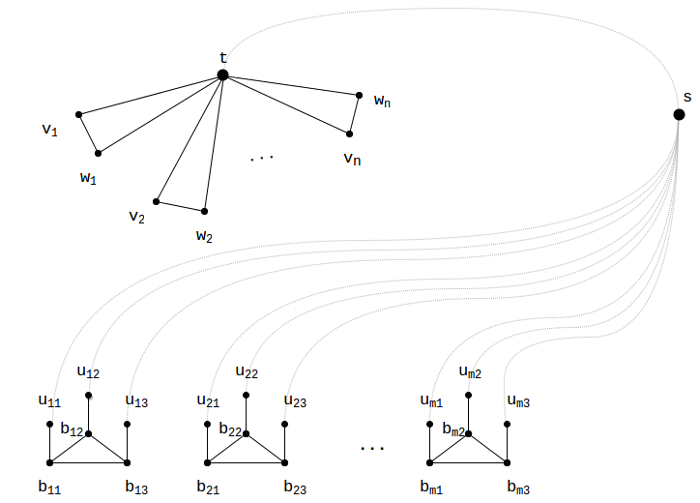
\includegraphics[width=14cm, height=9cm]{./graphics/3color_npcomplete.jpg}
			\end{center}

			\vspace{3mm}
			\underline{Construcción del grafo:}
				\begin{itemize}
					\item Dado un literal \textit{l}, definimos:
						\begin{equation*}
							\psi(l) =
	  					\left \lbrace
			  			\begin{array}{l}
	    				 	v_{k} \; \textup{ si } l = x_{k} \\
	    		 			w_{k} \textup{ si } l = \overline{x_{k}}
			  			\end{array}
	  					\right.
						\end{equation*}
					\item Vértices:
						\[ V(G) = \lbrace s, t \rbrace \cup \lbrace v_{1} \dotsc v_{n}, w_{1} \dotsc w_{n} \rbrace \; \cup \]
						\[ \qquad \qquad \; \; \; \; \lbrace \mu_{i, 1}, \mu_{i, 2}, \mu_{i, 3}, b_{i, 1}, b_{i, 2}, b_{i, 3} \rbrace_{i = 1}^{m}  \]
					\item Aristas:
						\[ E(G) = \lbrace s t \rbrace \cup \lbrace t v_{i}, t w_{i}, v_{i} w_{i} \rbrace_{i = 1}^{n} \; \cup \lbrace s \mu_{i, j} \rbrace_{i = 1, \; \; j = 1, 2, 3}^{m} \cup F \]
						\[ \cup \; \lbrace b_{i, 1} b_{i, 2}, b_{i, 1} b_{i, 3}, b_{i, 2} b_{i, 3}, b_{i, 1} \mu_{i, 1}, b_{i, 2}, \mu_{i, 2}, b_{i, 3} \mu_{i, 3} \rbrace_{i = 1}^{m}\]
						\par Donde:
						\[ F = \lbrace \mu_{i, j} \psi(l_{i, j}) \rbrace_{i = 1, \; \; j = 1, 2, 3}^{m}\]
				\end{itemize}

				\begin{equation*}
					\textup{ G tiene: }
	  				\left \lbrace
			  		\begin{array}{l}
	    				2 + 2n + 6m \textup{ vértices} \\
	    				1 + 3n + 3m+ 3m + 6m \textup{ aristas}
			  		\end{array}
	  				\right\rbrace
						\Rightarrow \textup{ G es polinomial}
				\end{equation*}

			\pagebreak
			\begin{tabular}{|c|} \hline $\Leftarrow$ \\\hline \end{tabular}
				\par Suponemos $\chi(G) \leq 3$ y construiremos un $\overrightarrow{b}$ tal que $B(\overrightarrow{b}) = 1$. Como G tiene triángulos, si $\chi (G) \leq 3$, entonces debe ser $\chi (G) = 3$. Por lo tanto, existe un coloreo C de G con 3 colores.
				\vspace{3mm}
				\par Definición:
				\begin{equation*}
					b_{k} =
		  		\left \lbrace
		  		\begin{array}{l}
		    		1 \textup{ si } C(v_{k}) = C(s) \\
		    		0 \textup{ si } C(v_{k}) \neq C(s)
		  		\end{array}
		  		\right.
				\end{equation*}
				\par Para probar $B(\overrightarrow{b}) = 1$ debemos probar que $D_{i}(\overrightarrow{b}) = l_{i, 1} \vee l_{i, 2} \vee l_{i, 3} = 1 \; \forall \; i$.
				\par Sea $i \in \lbrace	1, 2, \dotsc m \rbrace$, como $ \lbrace b_{i, 1}, b_{i, 2}, b_{i, 3} \rbrace$ es un triángulo, entonces deben aparecer los 3 colores. Es decir, $\exists j : C(b_{i, j}) = C(t)$
				\vspace{3mm}
				\par Luego:
				\begin{equation*}
		  		\left.
		  		\begin{array}{l}
		    		(1) \; \mu_{i, j} b_{i, j} \in E(G) \Rightarrow C(\mu_{i, j}) \neq C(b_{i, j}) = C(t) \\
		    		(2) \; \mu_{i, j} s \in E(G) \Rightarrow C(\mu_{i, j}) \neq C(s) \\
		    		(3) \; s t \in E(G) \Rightarrow C(s) \neq C(t)
		  		\end{array}
		 			\right\rbrace
		 			\Rightarrow C(\mu_{i, j}) = \textup{ TERCER COLOR}
				\end{equation*}

				\par Por otro lado:
				\begin{equation*}
		  		\left.
		  		\begin{array}{l}
		    	 	(1) \; \mu_{i, j} \psi(l_{i, j}) \in E(G) \Rightarrow C(\psi(l_{i, j})) \neq \textup{ TERCER COLOR} \\
		    	 	(2) \; \psi(l_{i, j}) t \in E(G) \Rightarrow C(\psi(l_{i, j}) \neq C(t)
		  		\end{array}
		 		 	\right\rbrace
		 			\Rightarrow C(\psi(l_{i, j}) = C(s)
				\end{equation*}

				\begin{itemize}
					\item \underline{Caso (1):}
						\begin{equation*}
							l_{i, j} = x_{k} \Rightarrow
		  					\left\lbrace
							\begin{array}{l}
	  		 					l_{i, j}(\overrightarrow{b}) = b_{k} \\
								\psi(l_{i, j}) = v_{k}
							\end{array}
							\right.
						\end{equation*}
						
						\par Entonces:
						\begin{eqnarray}
							\nonumber C(v_{k}) &=& C(s) \Rightarrow b_{k} = 1 \\
							\nonumber \therefore l_{i, j}(\overrightarrow{b}) &=& 1 \Rightarrow D_{i}(\overrightarrow{b}) = 1
						\end{eqnarray}
					\item \underline{Caso (2):}
						\begin{equation*}
							l_{i, j} = \overline{x_{k}} \Rightarrow
		  					\left\lbrace
							\begin{array}{l}
	  		 					l_{i, j}(\overrightarrow{b}) = 	\overline{b_{k}} \\
								\psi(l_{i, j}) = w_{k}
							\end{array}
							\right.
						\end{equation*}

						\par Entonces:
						\begin{equation*}
		  				\left.
		  				\begin{array}{l}
		    		 		C(w_{k}) = C(s) \\
		    		 		v_{k} w_{k} \in E(G)
		  				\end{array}
		 			 		\right\rbrace
		 			 		\Rightarrow C(v_{k}) \neq C(s) \therefore b_{k} = 0
						\end{equation*}
						$\qquad\qquad\qquad\qquad\qquad$
						$\therefore \overline{b_{k}} = 1 \Rightarrow D_{i}(\overrightarrow{b}) = 1$
				\end{itemize}

			\pagebreak
			\begin{tabular}{|c|} \hline $\Rightarrow$ \\\hline \end{tabular}
				\par Acá asumimos que $\exists \overrightarrow{b} : B(\overrightarrow{b}) = 1 \Rightarrow \forall i, \; D(\overrightarrow{b}) = 1 \Rightarrow$ \begin{tabular}{|c|} \hline $\forall i \; \exists j : l_{i, j}(\overrightarrow{b}) = 1$ \\ \hline \end{tabular} $(\star)$. Debemos construir un coloreo propio con 3 colores.
				\vspace{3mm}
				\par Definimos:
				\begin{equation*}
		  		\left.
		  		\begin{array}{l}
		    		C(s) = \textup{ BLANCO} \\
		    		C(t) = \textup{ AZUL}
		  		\end{array}
		 			\right\rbrace
		 			\Rightarrow s t \textup{ No Crea Problemas (NCP)}
				\end{equation*}
				\begin{equation*}
					C(v_{k}) =
					\left\lbrace
		  		\begin{array}{l}
		    		\textup{BLANCO \; si } b_{k} = 1 \\
		    		\textup{NEGRO \; \; si } b_{k} = 0
					\end{array}
		 			\right\rbrace
		 			\Rightarrow \underbrace{v_{k}}_{B \; o \; N} \underbrace{w_{k}}_{B \; o \; N} \textup{ NCP}
				\end{equation*}
				\begin{equation*}
					C(w_{k}) =
		  		\left\lbrace
					\begin{array}{l}
	  		 		\textup{NEGRO \; \, si } b_{k} = 1 \\
	  		 		\textup{BLANCO \; si } b_{k} = 0
					\end{array}
				 	\right\rbrace
				 	\Rightarrow \underbrace{v_{k}}_{B o N} \underbrace{t}_{A}  \textup { y } \underbrace{w_{k}}_{B o N} \underbrace{t}_{A} \textup{ NCP}
				\end{equation*}

				\par Falta colorear las garras. Dado \textit{i}, tomemos el \textit{j} de $(\star )$ y definimos:
				\begin{equation*}
					C(\mu_{i, r}) =
		  		\left\lbrace
					\begin{array}{l}
	  		 		\textup{NEGRO \; \; si } r = j \\
	  		 		\textup{AZUL \qquad si } r \neq j
					\end{array}
				 	\right\rbrace
				 	\Rightarrow \underbrace{\mu_{i, r}}_{N \; o \; A} \underbrace{s}_{B} \textup{ NCP } \forall r
				\end{equation*}

				\begin{itemize}
					\item \underline{Caso $r \neq j$:} $\qquad \underbrace{\mu_{i, r}}_{A} \underbrace{\psi(l_{i, r})}_{B \; o \, N} \Rightarrow$ NCP
					\item \underline{Caso $r = j$:}
						\begin{itemize}
							\item Caso (1):
								\begin{equation*}
									l_{i, j} = x_{k} \Rightarrow
		  							\left\lbrace
									\begin{array}{l}
	  		 							l_{i, j}(\overrightarrow{b}) = b_{k} = 1 \Rightarrow C(v_{k}) = \textup{ BLANCO} \\
	  		 							\psi(l_{i, j}) = v_{k}	\Rightarrow \mu_{i, j} \psi(l_{i, j}) = \underbrace{\mu_{i, j}}_{N} \underbrace{v_{k}}_{B} \textup{ NCP}
									\end{array}
									\right.
								\end{equation*}

							\item Caso (2):
								\begin{equation*}
									l_{i, j} = \overline{x_{k}} \Rightarrow
		  							\left\lbrace
									\begin{array}{l}
	  		 							l_{i, j}(\overrightarrow{b}) = \overline{b_{k}} = 1 \Rightarrow b_{k} = 0 \Rightarrow C(w_{k}) = \textup{ BLANCO} \\
										\psi(l_{i, j}) = w_{k}	\Rightarrow \mu_{i, j} \psi(l_{i, j}) = \underbrace{\mu_{i, j}}_{N} \underbrace{w_{k}}_{B} \textup{ NCP}
									\end{array}
									\right.
								\end{equation*}
						\end{itemize}
				\end{itemize}

				\par Quedan las bases:
				\begin{equation*}
					C(b_{i, r}) =
				  \left\lbrace
		  		\begin{array}{l}
		    		\textup{AZUL \qquad \qquad\qquad \; \; \; si } r = j \\
		    		\textup{BLANCO o NEGRO \; \; si } r \neq j \\
		    		\textup{NEGRO o BLANCO \; \; si } r \neq j
		  		\end{array}
		 			\right.
				\end{equation*}

				\par Es decir, le damos el color AZUL al $b_{i, j}$ y los otros dos los coloreamos uno NEGRO y uno BLANCO, de modo que:
				\begin{itemize}
					\item $\lbrace b_{i, 1}, b_{i, 2}, b_{i, 3} \rbrace \textup{ NCP}$
			 		\item $\underbrace{b_{i, j}}_{A} \underbrace{\mu_{i, j}}_{N} \textup{ NCP}$
			 		\item $\underbrace{b_{i, r}}_{B \; o \; N} \underbrace{\mu_{i, r}}_{A} \textup{ NCP}$
				\end{itemize}

		\QED


\begin{thebibliography}{X}
\bibitem{Baz} \textsc{Maximiliano Illbele},
<<Resumen de Discreta II, 16 de agosto de 2012>>,
\textit{FaMAF, UNC}.
\bibitem{Baz} \textsc{Lucia Pappaterra},
<<Resumen de Discreta II, 2014>>,
\textit{FaMAF, UNC}.
\bibitem{Baz} \textsc{Marcos Modenesi},
<<Resumen de Discreta II, 2016>>,
\textit{FaMAF, UNC}.
\bibitem{Baz} \textsc{Agustín Curto},
<<Carpeta de Clase, 2016>>,
\textit{FaMAF, UNC}.
\end{thebibliography}

\vspace{\fill}
\begin{center}
Por favor, mejorá este documento en github

\includegraphics[width=1cm]{graphics/github.png} \\
https://github.com/ResumenesFaMAF/resumenDiscreta2
\end{center}
\end{document}
